\subsection{Consideraciones generales}

Para armar los circuitos propuestos por la cátedra se dispone de un
amplificador operacional LM-833N. Los datos más importantes a considerar
vistos en la hoja de datos son los siguientes:
\begin{itemize}
    \item $A_{vol}$ = $110dB$ 
    \item BWP = $15 MHz$
    \item $\omega_b$ = $47 Hz$
\end{itemize}   

\subsection{Circuito Derivador}

A continuación, se realiza el análisis sobre el circuito derivador planteado
por la cátedra utilizando un amplificador operacional $LM833$ aplicado en el siguiente circuito.
\begin{figure}[H]
    \centering
    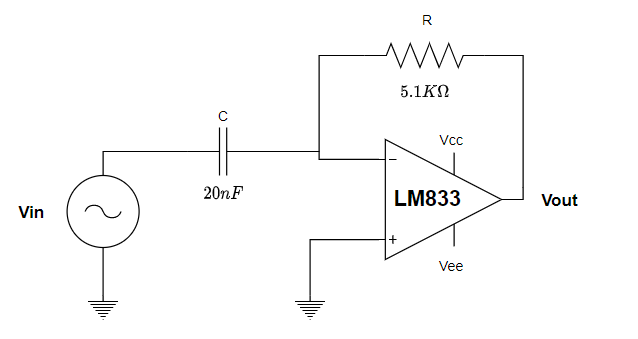
\includegraphics[width=0.6\textwidth]{../Ejercicio3-CircuitoIntegradoresyDerivadores/Imagenes/Derivador/circuito_derivador.png}
    \caption{Circuito derivador implementado con Opamp}
\end{figure}
Se obtuvo una diferencia entre los valores teóricos y medidos de los componentes 
que se muestran en la siguiente tabla.
\begin{table}[H]
    \centering
    \begin{tabular}{|c|c|c|}
    \hline
                 & C       & R             \\ \hline
    Teórico      & 20 nF   & 5k1$\Omega$   \\ \hline
    Medido       & 18.8 nF & 5.27 $\Omega$ \\ \hline
    $\epsilon_r$ & 6.4\%    & 3.3\%          \\ \hline
    \end{tabular}
    \end{table}


\subsubsection{Respuesta en frecuencia}
Consiguientemente, se procede a calcular la transferencia de tensión entra
la entrada y salida del circuito. \par 
En condición ideales, se considera que la ganancia del
amplificador operacional es infinita, por lo que, basándonos en 
su ecuación característica (\ref{eq_opamp}), se puede asegurar que para 
mantener la relación $V^+=V^-$, la resta entre ambos voltajes va a tender a 0.
\vspace{2mm}
\begin{equation}
    V_{out}=A_0(V^+-V^-)  \rightarrow V_{out}=-A_0V^-
    \label{eq_opamp}
\end{equation}
\vspace{2mm}
Por lo tanto, se pueden escribir a las corrientes del circuito como:
\vspace{2mm}
\begin{equation}
    I_1=\frac{V{in}}{X_c}=V_{in}\$C_1 \indent \indent I_2=\frac{V_{out}}{R}
    \label{eq_avol_ideal}
\end{equation}
\vspace{2mm}
Considerando que $V^-=0$ y que $I_1=I_2$ se logra llegar a la transferencia bajo 
condiciones ideales:
\vspace{2mm}
\begin{equation}
    H(\$)=\frac{V_{out}}{V_{in}}=-R\$C
    \label{trans_ideal}
\end{equation}
\vspace{2mm}
Por otro lado, considerando a $A_{vol}$ finito se vuelve indispensable reformular las
ecuaciones vistas en \ref{eq_avol_ideal} ya que al considerar un $A_{vol}$ que no 
tiende a infinito se vuelve imposible asegurar que la tensión $V^-$ sea nula. Bajo 
las nuevas circunstancias se obtienen:
\vspace{2mm}
\begin{equation}
    I_1=\frac{V{in}-V^-}{X_c}=(V_{in}-V^-)\$C_1 \indent \indent I_2=\frac{V_{out}-V^-}{R}
    \label{eq_avol_noideal}
\end{equation}
\vspace{2mm}
Utilizando \ref{eq_opamp} y \ref{eq_avol_noideal} se puede despejar la transferencia
como:
\vspace{2mm}
\begin{equation}
    H_1(\$)=\frac{V_{out}}{V_{in}}=\frac{-R\$C}{1+\left(\frac{R\$C+1}{A_0}\right)}=- \left(\frac{A_{vol}RC}{A_{vol}+1}\right)\frac{\$}{ \left(\frac{\$}{\frac{A_{vol}+1}{RC}}\right)+1}
    \label{trans_no_ideal}
\end{equation}
\vspace{2mm}
Se puede validar este ecuación considerando:
 $$\lim_{A_0\to\infty} H_1(\$)=H(\$)$$
Obteniéndose la transferencia en condiciones ideales vista en \ref{trans_ideal}. \par
Para finalizar se realiza un análisis considerando $A_{vol}$ variante en frecuencia
debido a la presencia de un polo dominante que le da una respuesta en frecuencia 
característica de un filtro pasa-bajos. La dependencia en frecuencia de la ganancia
del opamp está dada por la siguiente fórmula:
\vspace{2mm}
\begin{equation}
    A_v(\$)=\frac{A_0}{1+\frac{\$}{w_b}}
    \label{a_vol_frec}
\end{equation}
\vspace{2mm}
Siendo $A_0$ la ganancia en lazo abierto del opamp y $w_b$ la frecuencia del polo dominante,
 frecuencia para la cual el dispositivo atenúa 3 dB. \par 
 Reemplazando (\ref{a_vol_frec}) en (\ref{trans_no_ideal}) se obtiene:
 \vspace{2mm}
 \begin{equation}
    H_2(\$)=\frac{-R\$C}{\left(1+\frac{1}{A_0}\right)+\$\left(\frac{RCw_b+1}{w_bA_0}\right)+\frac{\$^2}{\frac{w_bA_0}{RC}}}
    \label{trans_frec}
\end{equation}
\vspace{2mm}
Esta ecuación se puede dividir según su ganancia ideal $G_I$ y su factor de corrección
$F_c$ de la siguiente forma:
\vspace{2mm}
\begin{equation*}
   G_I=-R\$C \indent \indent F_c={\left(1+\frac{1}{A_0}\right)+\frac{\$(RCw_b+1)}{w_bA_0}+\frac{R\$^2C}{w_bA_0}}
   \label{trans_frec}
\end{equation*}
\vspace{2mm}
Siguiendo el mismo procedimiento aplicado para $H_1(\$)$, se puede formular:
 $$\lim_{A_0\to\infty} H_2(\$)=\lim_{A_0\to\infty} G_IF_C=G_I=H(\$)$$

Las expresiones obtenidas se plasman en el siguiente gráfico, pudiéndose 
observar una mayor precisión a medida que se usan modelos más realistas
sin consideraciones ideales.

\begin{figure}[H]
    \centering
    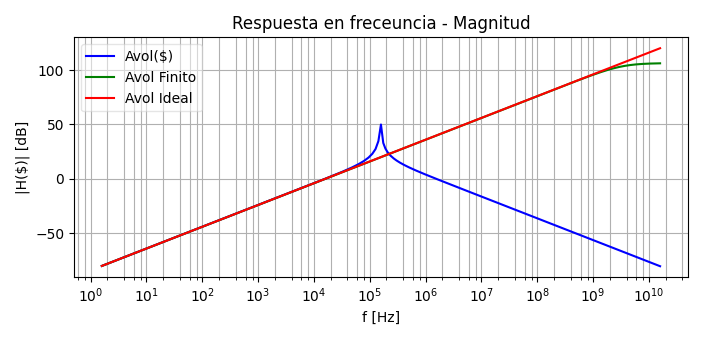
\includegraphics[width=0.6\textwidth]{../Ejercicio3-CircuitoIntegradoresyDerivadores/Imagenes/Derivador/bode_derivador_magnitud.png}
    \caption{Respuesta en frecuencia teóricas - Módulo}
\end{figure}
\begin{figure}[H]
    \centering
    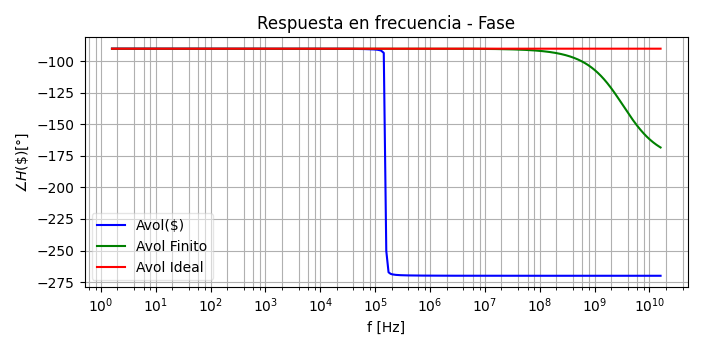
\includegraphics[width=0.6\textwidth]{../Ejercicio3-CircuitoIntegradoresyDerivadores/Imagenes/Derivador/bode_derivador_fase.png}
    \caption{Respuesta en frecuencia teóricas - Fase}
\end{figure}

A mayores frecuencias se puede observar un par de polos conjugados en el modelo de 
$A_{vol}$ finito, cuya frecuencia se puede despejar de la función transferencia \ref{trans_frec}, tomando 
la misma el siguiente valor:
\begin{equation}
    \vspace{2mm}
    f_0=\frac{1}{2\pi}\sqrt{\frac{w_b(A_0+1)}{RC}}\approx 154.5KHz
    \vspace{2mm}
\end{equation}
Por otro lado, al considerar que el sobrepico presente es de magnitud considerable
y que el cambio de fase es rápido, se esperara un $\xi$ relativamente bajo que 
indique un circuito sumamente subamortiguado. Dicho valor se puede despejar
de  \ref{trans_frec} como el valor anterior:
\begin{equation}
    \vspace{2mm}
    \xi=\frac{w_0(RCw_b+1)}{2A_0w_b}\approx \num{5.22e-3}
    \vspace{2mm}
\end{equation}
Tomando en consideración $A{vol}$ finito, se observa la transferencia hallada 
en \ref{trans_no_ideal}. De la misma se desprende la presencia de un polo en:
\begin{equation}
    \vspace{2mm}
    f=\frac{A{vol}+1}{RC}\approx 508MHz
    \vspace{2mm}
\end{equation}
Esto coincide con lo visto en el gráfico ya que aproximadamente una década por 
debajo empieza un desfasaje de -90$^\circ$ que termina una década por encima.
Bajo lo anteriormente expuesto, los cálculos despejados de la ecuación coinciden
con lo visto en los gráficos. A fines prácticos, dicho polo no es de interés 
ya que el circuito no será utilizados a altas frecuencias.\par 
A continuación, se presentan la respuesta en frecuencia tanto simulada como medida 
en el circuito.


\begin{figure}[H]
    \centering
    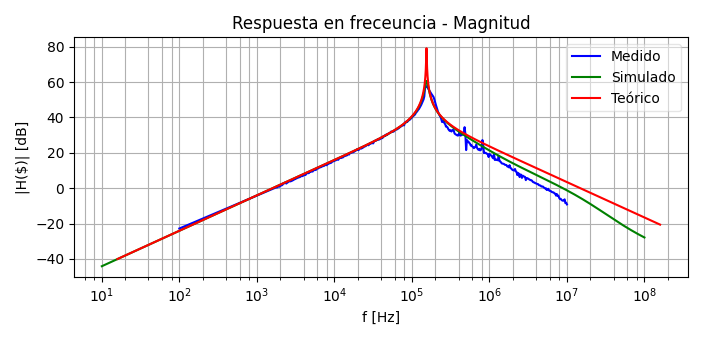
\includegraphics[width=0.6\textwidth]{../Ejercicio3-CircuitoIntegradoresyDerivadores/Imagenes/Derivador/comparacion_magnitud.png}
    \caption{Comparación respuesta en frecuencia - Módulo}
    \label{graph_trans_mag}
\end{figure}
\begin{figure}[H]
    \centering
    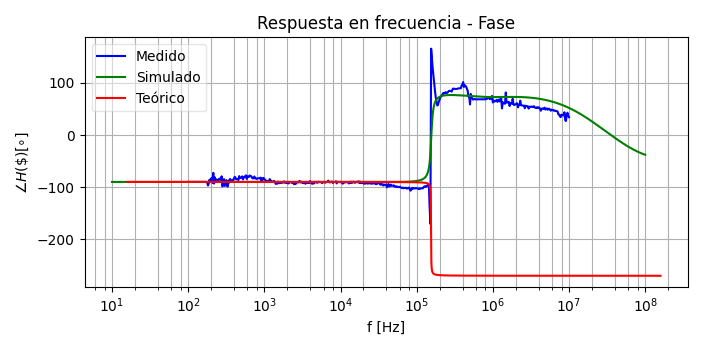
\includegraphics[width=0.6\textwidth]{../Ejercicio3-CircuitoIntegradoresyDerivadores/Imagenes/Derivador/comparacion_fase.png}
    \caption{Comparación respuesta en frecuencia - Fase}
    \label{graph_trans_pha}
\end{figure}
Observando las figuras anteriores, se hace presente una correcta correlación entre
el modelo teórico, la experiencia simulada y su realización empírica.
Al ser de interés su comportamiento como derivador el circuito tendrá que ser usado a una 
frecuencia inferior a los $100 KHz$, frecuencias para las cuales el comportamiento es 
consistente para los tres casos. \par 

Consideramos pertinente comentar los problemas presentes al intentar medir el sobrepico de la respuesta en frecuencia
debido a que el equipo \textit{Electronic Explorer} realiza el barrido en frecuencia usando una señal de entrada configurable
de un $1V$, la cual al estar en el pico, es amplificada en más de $40dB$. Dicha amplificación
nos producía que el sistema se fuera de escala, siendo imposible 
detectarlo. Por otro lado, al experimentar con una tensión de entrada menor, la señal ya se perdía junto con
el ruido  de alta frecuencia presente en el sistema. \par  Para sortear dicho problema
se implementó el circuito mostrado en \ref{circuito_medidor_derivador}, utilizando un atenuador de $40dB$ más un buffer,
de manera tal de separar las etapas y que no se carguen entre si. De esta manera, se logró medir efectivamente el pico 
postulado tanto en el modelo simulado como el teórico.

\begin{figure}[H]
    \centering
    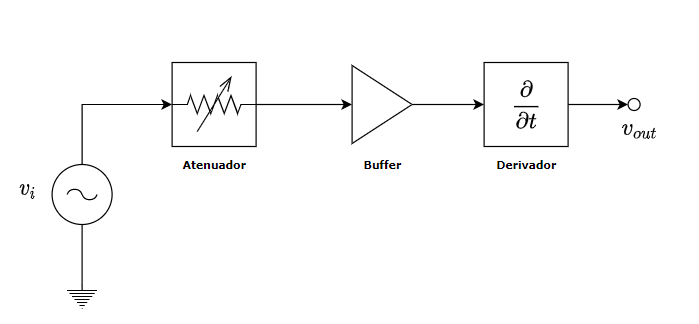
\includegraphics[width=0.6\textwidth]{../Ejercicio3-CircuitoIntegradoresyDerivadores/Imagenes/Derivador/circuito_medidor.png}
    \caption{Circuito de medición para la respuesta en frecuencia}
    \label{circuito_medidor_derivador}
\end{figure}



\subsubsection{Impedancia de entrada}

Para calcular la impedancia de entrada se procede con el mismo análisis que para 
la transferencia, considerando los distintos modelos para la ganancia del opamp. Para el primer 
caso, el hecho de poseer una $A_{vol}$ de carácter infinito induce una tierra virtual 
perfecta en $V^-$, permitiendo llegar a:

\vspace{2mm}
\begin{equation}
   Z_{in_1}=\frac{V_i}{I_1}=\frac{1}{\$C} 
    \label{zin_ideal}
\end{equation}
\vspace{2mm}
Por otro lado, al considerar una ganancia finita, se puede despejar de \ref{eq_avol_noideal} y \ref{eq_opamp}
la impedancia de entrada para el caso no ideal.

\vspace{2mm}
\begin{equation}
    Z_{in2}=\frac{V_i}{I_1}=\frac{1}{\$C}\frac{1}{\left(1-\frac{R\$C}{1+A_0+R\$C}\right)} 
    \label{zin_avol_ideal}
\end{equation}
\vspace{2mm}

Se puede validar este ecuación considerando:
 $$\lim_{A_0\to\infty} Z_{in_2}=Z_{in_1}$$
Para finalizar, se reemplaza la variación en frecuencia del opamp dada por \ref{a_vol_frec}, obteniéndose:

\vspace{2mm}
\begin{equation}
    Z_{in3}=\frac{V_i}{I_1}=\frac{1}{\$C}\frac{1}{1-\frac{R\$C+\frac{R\$^2C}{w_b}}{\frac{R\$^2C}{w_b} +\$(RC+\frac{1}{w_b})+(1+A_0)}} 
    \label{zin_avol_frec}
\end{equation}
\vspace{2mm}

También, se puede validar este ecuación considerando:
 $$\lim_{A_0\to\infty} Z_{in_3}=Z_{in_1}$$

Las expresiones obtenidas se plasman en el siguiente gráfico, pudiéndose 
observar una mayor precisión a medida que se usan modelos más realistas
sin consideraciones ideales.

\begin{figure}[H]
    \centering
    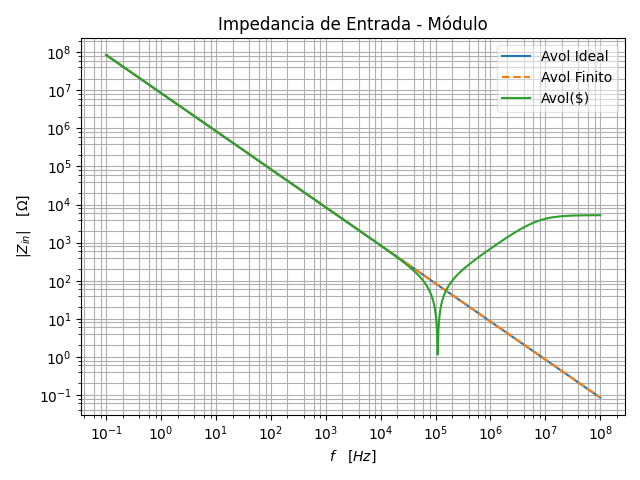
\includegraphics[width=0.6\textwidth]{../Ejercicio3-CircuitoIntegradoresyDerivadores/Imagenes/Derivador/Zin/impedancia_teo_mag.png}
    \caption{Impedancias de entrada teóricas - Módulo}
\end{figure}
\begin{figure}[H]
    \centering    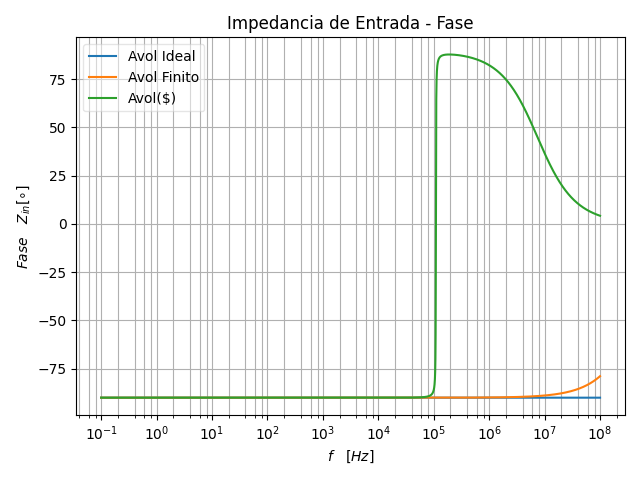
\includegraphics[width=0.6\textwidth]{../Ejercicio3-CircuitoIntegradoresyDerivadores/Imagenes/Derivador/Zin/impedancia_teo_fase.png}
    \caption{Impedancias de entrada teóricas - Fase}
\end{figure}

A continuación, se presentan la impedancia de entrada tanto simulada como teórica 
en el circuito.


\begin{figure}[H]
    \centering
    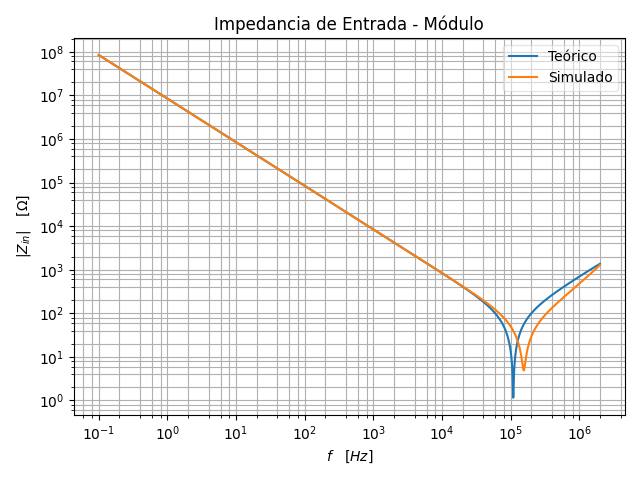
\includegraphics[width=0.6\textwidth]{../Ejercicio3-CircuitoIntegradoresyDerivadores/Imagenes/Derivador/Zin/Z_in_comparacion_mod.png}
    \caption{Comparación Impedancias de entrada - Módulo}
    \label{graph_z_in_mag}
\end{figure}
\begin{figure}[H]
    \centering
    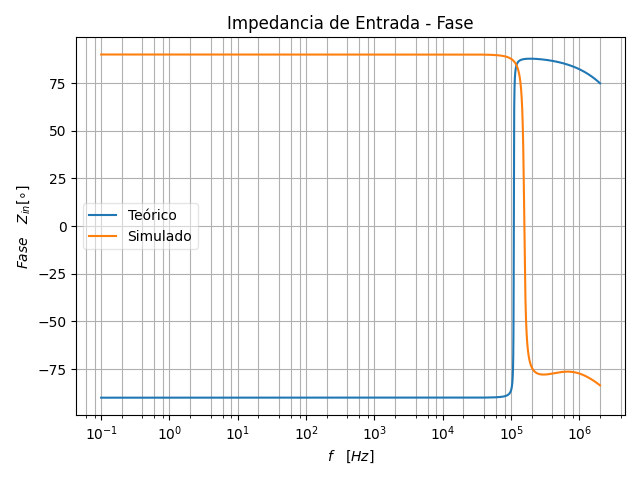
\includegraphics[width=0.6\textwidth]{../Ejercicio3-CircuitoIntegradoresyDerivadores/Imagenes/Derivador/Zin/Z_in_comparacion_pha.png}
    \caption{Comparación Impedancias de entrada - Fase}
    \label{graph_z_in_pha}
\end{figure}
Observando las figuras anteriores, se puede observar una correcta correlación entre la impedancia de entrada 
y las transferencias obtenidas vistas en \ref{graph_trans_mag} y \ref{graph_trans_pha}. Al ponerse el capacitor
en corto alrededor de los $150KHZ$ ocurre el mínimo de impedancia, se observa la coincidencia de sobrepico 
en el gráfico de transferencia. Por otro lado, el sobrepico menos abrupto se debe a que el modelo 
simulado del capacitor contiene una resistencia serie o paralela que no permite que su impedancia se haga
realmente nula.

\subsubsection{Respuesta ante una senoidal}
A continuación, previo al análisis de la respuesta del circuito ante una senoidal, se hace una análisis de las 
frecuencias de operación del circuito que servirán como base para posteriores análisis. \par 
Como primer consideración, se puede afirmar que el comportamiento como derivador, la zona de estudio sobre 
la cual hay interés, coincide para los tres modelos propuestos, por lo tanto, se toma el modelo más sencillo 
 de transferencia dado por \ref{trans_ideal}, considerando un $A_{vol}$ infinito. En dicho caso, el modulo
de la transferencia será proporcional a la frecuencia, estando dado por:
\vspace{2mm}
\begin{equation}
    |H(f)|=\frac{CRf}{2\pi}
    \label{frec_unitaria}
\end{equation}
\vspace{2mm}

Despejando de la función transferencia \ref{trans_ideal} se puede observar que la frecuencia de ganancia 
unitaria del circuito está dada por: 

\vspace{2mm}
\begin{equation}
    f_t=\frac{1}{2\pi RC} \approx 1.6KHz
    \label{frec_unitaria}
\end{equation}
\vspace{2mm}

Dicho valor coincide con el observable en el gráfico \ref{graph_trans_mag}. \par 
Por debajo de $f_t$ se podrán lograr atenuaciones de hasta $50dB$ a frecuencias bajas y ganancias de hasta 
$40dB$ justo antes del polo dominante del circuito, punto en el cual el derivador deja de cumplir su función. \par 
Habiendo realizado todas las consideraciones anteriores, se analiza la respuesta del sistema ante una señal senoidal
de frecuencia $1.6HKz$, esperando observar su comportamiento derivador con una ganancia unitaria.

\begin{figure}[H]
    \centering
    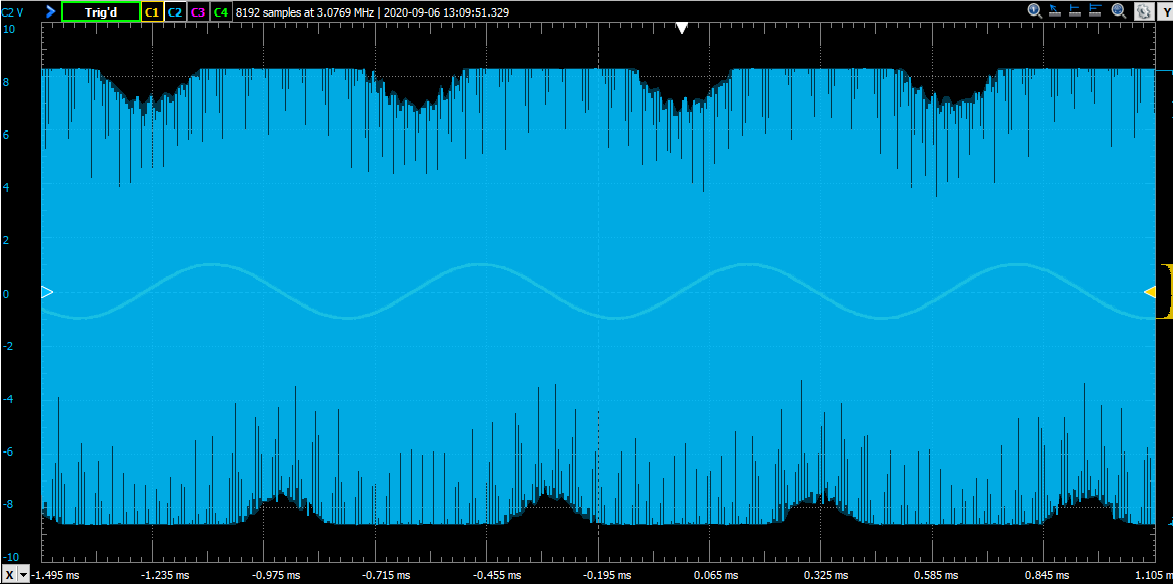
\includegraphics[width=0.6\textwidth]{../Ejercicio3-CircuitoIntegradoresyDerivadores/Imagenes/Derivador/ruido_alto_f.png}
    \caption{Ruido de alta frecuencia generado por el THD del generador}
    \label{thd}
\end{figure}
Lamentablemente, no se observa lo esperado debido a que la experiencia empírica dista en gran medida del modelo 
teórico, esto se debe a factores y limitaciones que no estamos considerando. Para este caso en particular, 
lo que está sucediendo es que el generador de funciones del equipo no es un generador ideal,
 siendo incapaz de ofrecer 
una señal que sólo tenga componentes en la frecuencia deseada, poseyendo una composición armónica
 parásita denominada distorsión armónica
\textit{(THD)}. Para este caso en particular, la THD del generador es alta. \par 
 Los componentes parásitos de alta frecuencia de la señal se ven amplificados según 
la transferencia vista en \ref{graph_trans_mag}, dicho análisis coincide con el visto mediante en el analizador 
de espectro del equipo en el siguiente gráfico. 
\begin{figure}[H]
    \centering
    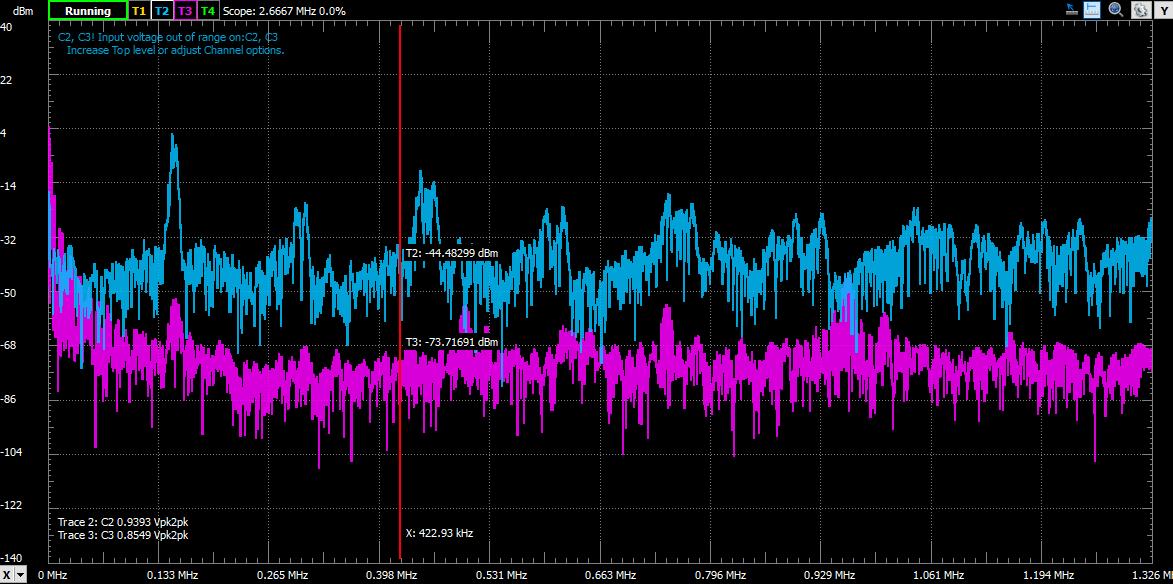
\includegraphics[width=0.6\textwidth]{../Ejercicio3-CircuitoIntegradoresyDerivadores/Imagenes/Derivador/thd.png}
    \caption{Análisis espectral del THD}

\end{figure}
La señal azul es la observada en la salida del derivador mientras que la violeta es su correlativa a la entrada.
A simple vista, los componentes parásitos de la señal de entrada no son distinguibles del piso de ruido, sin embargo
para valores cercanos al pico de transferencia se produce una gran amplificación de los mismos, generando el ruido
observado en  \ref{thd}. \par 
Por ende, para resolver este problema se utiliza un filtro pasa-bajos a la entrada para filtrar los componentes 
parásitos de alta frecuencia provistos por la fuente.  El sistema de medición utilizado es el siguiente:

\begin{figure}[H]
    \centering
    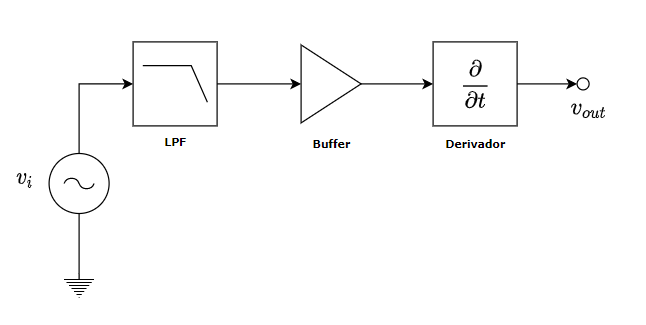
\includegraphics[width=0.6\textwidth]{../Ejercicio3-CircuitoIntegradoresyDerivadores/Imagenes/Derivador/circuito_thd.png}
    \caption{Circuito implementado para reducir el ruido}

\end{figure}
La frecuencia de corte será una década por encima de la frecuencia de la senoidal buscada, en este caso $16KHz$. 
Por otro lado,
habrá que tener en consideración el desfasaje agregado de $-90^\circ$. \par 
Implementado este sistema, se puede observar lo siguiente:

\begin{figure}[H]
    \centering
    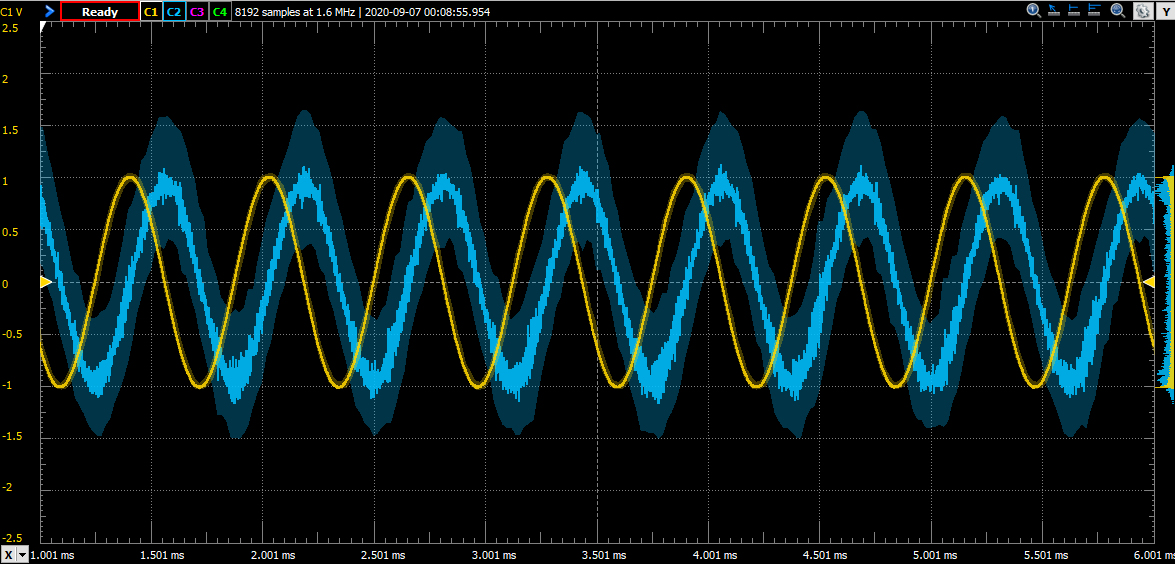
\includegraphics[width=0.6\textwidth]{../Ejercicio3-CircuitoIntegradoresyDerivadores/Imagenes/Derivador/captura_sen.png}
    \caption{Respuesta medida del sistema ante una señal senoidal de 1K6 Hz}

\end{figure}

A continuación, se grafica la comparación entre el la respuesta del sistema 
teórico, medido y simulado.
\begin{figure}[H]
    \centering
    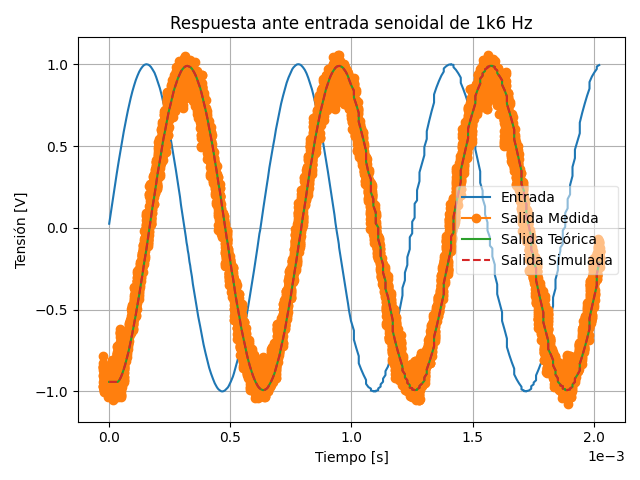
\includegraphics[width=0.6\textwidth]{../Ejercicio3-CircuitoIntegradoresyDerivadores/Imagenes/Derivador/rta_sen_1k6.png}
    \caption{Comparación de la respuesta del sistema ante una señal senoidal de 1K6 Hz}

\end{figure}
Se puede apreciar una excelente correlación entre los tres sistemas planteados.

Para continuar con el análisis del derivador implementado, se estudiará
la respuesta del sistema ante una señal triangular. Para este caso,
se elimina el filtro pasa-bajos ya que deformaría en gran medida 
la señal de la entrada. \par 
Como primer análisis, se elige una señal de amplitud $1V$ y frecuencia 
$1.6 KHz$, la misma coincide con su frecuencia de ganancia unitaria por lo que
se esperará que la señal de salida no vea modificada su amplitud. De otra manera,
lo que si se verá modificado será la forma de la señal, esperando obtener
una señal cuadrada a la salida.

\begin{figure}[H]
    \centering
    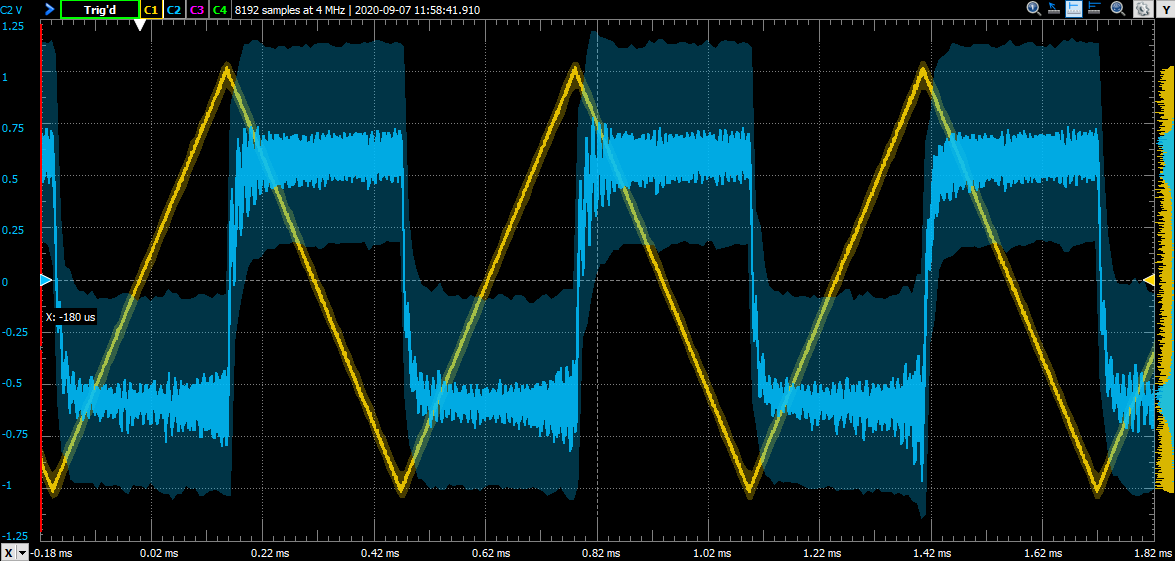
\includegraphics[width=0.6\textwidth]{../Ejercicio3-CircuitoIntegradoresyDerivadores/Imagenes/Derivador/trian_1k6.png}
    \caption{Respuesta medida del sistema ante una señal triangular de 1K6 Hz}

\end{figure}
Teniendo en consideración lo observado en la imagen anterior, se puede sostener que se obtiene 
lo esperado, una señal cuadrada de igual magnitud. El gran nivel de ruido se debe a la presencia 
de componentes de alta frecuencia de la  triangular que son amplificados por el derivador. 

\begin{figure}[H]
    \centering
    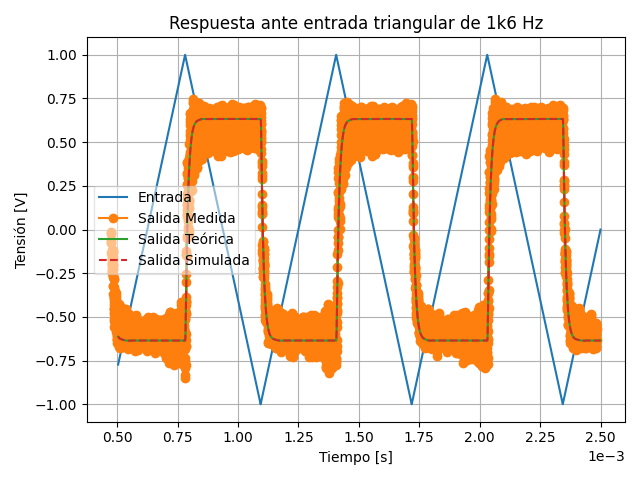
\includegraphics[width=0.6\textwidth]{../Ejercicio3-CircuitoIntegradoresyDerivadores/Imagenes/Derivador/rta_triangular_1k6.png}
    \caption{Comparación de la respuesta del sistema ante una señal triangular de 1K6 Hz}

\end{figure}

El siguiente caso a analizar es el de una señal triangular de amplitud de $1V$, pero con una frecuencia
que se encuentra una década por debajo de la frecuencia de ganancia unitaria, es decir, utilizaremos
una frecuencia de $160Hz$. Observando el gráfico de transferencia visto en \ref{graph_trans_mag}, es
de esperar una atenuación de $20dB$ en la señal de salida.

\begin{figure}[H]
    \centering
    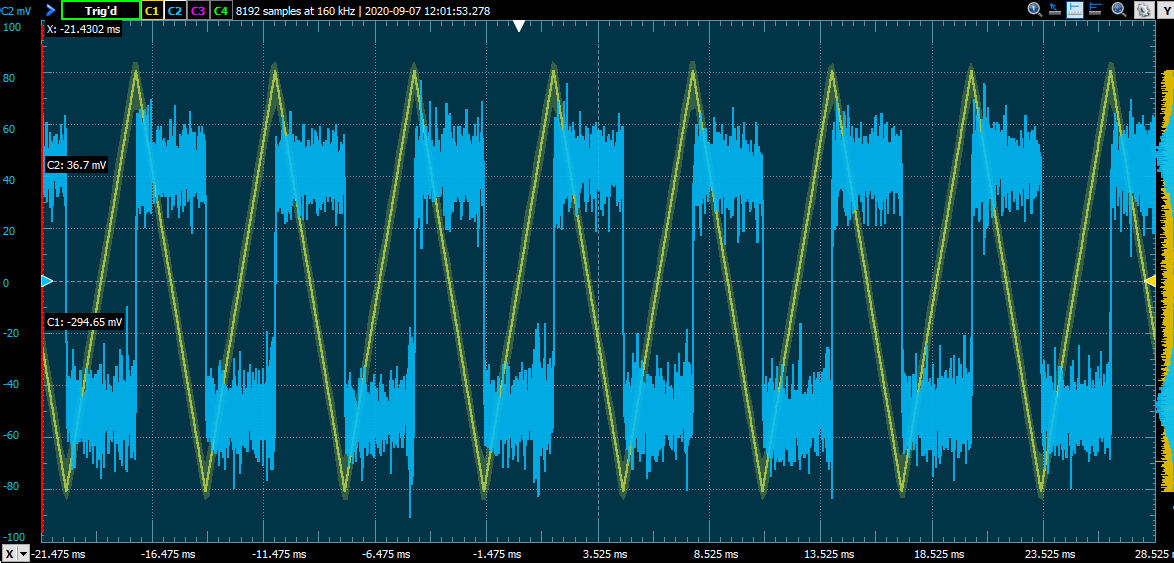
\includegraphics[width=0.6\textwidth]{../Ejercicio3-CircuitoIntegradoresyDerivadores/Imagenes/Derivador/trian_160.png}
    \caption{Respuesta medida del sistema ante una señal triangular de 160 Hz}
\end{figure}
La salida coincide con lo esperado, siendo una señal cuadrada de amplitud $100mV$. Por otro lado,
también se observa un mayor nivel de ruido, esto se debe a que el piso de ruido de alta frecuencia 
se hace más notorio al trabajar con amplitudes más pequeñas.
\begin{figure}[H]
    \centering
    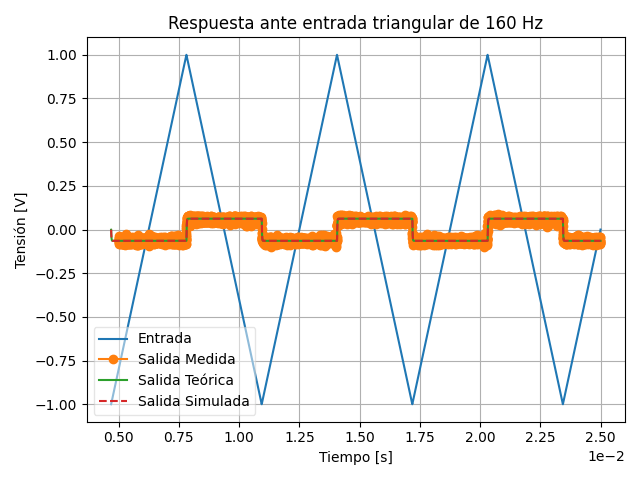
\includegraphics[width=0.6\textwidth]{../Ejercicio3-CircuitoIntegradoresyDerivadores/Imagenes/Derivador/rta_triangular_160.png}
    \caption{Comparación de la respuesta del sistema ante una señal triangular de 160 Hz}

\end{figure}


\subsubsection{Compensación}
En este apartado se realizará un análisis sobre la colocación de una resistencia de compensación
$R_C$ en el circuito para mejorar su funcionamiento, atenuando el sobrepico presente a altas 
frecuencias, alrededor de los $150 KHz$. \par 
Como se puede observar en las gráficas 
ya presentadas de $Z_{in}$ y $H(\$)$ (\ref{graph_trans_mag} y \ref{graph_z_in_mag}), el sobrepico
se debe a que la impedancia del capacitor se vuelve mínima, siendo equivalente a un cortocircuito, de
esta manera, la impedancia de entrada se hace casi cero, permitiendo una transferencia extremadamente alta.\par 
Para corregir dicho inconveniente, es necesario colocar una resistencia de bajo valor 
en serie con el capacitor del circuito 
mostrado previamente en \ref{circuito_medidor_derivador}. De esta manera, cuando la impedancia del capacitor
baje llegará un punto en el que la misma se haga del orden de la resistencia, evitando la situación de cortocircuito
y el sobrepico. Para este punto, el circuito se comportará como un inversor. \par 
Cuando nos referimos a bajo valor hacemos referencia a un valor tal que no afecte el funcionamiento 
normal del derivador, ya sea modificando su transferencia y/o impedancia de entrada. Para calcular el 
valor de resistencia a colocar, se analiza la impedancia del capacitor a dicha frecuencia, siendo la misma:
\vspace{2mm}
\begin{equation*}
    X_c=\frac{1}{2\pi*80KHz**18.88nF}\approx 100 \Omega
\end{equation*}
\vspace{2mm}
Basándonos en el razonamiento anterior, se utilizará una resistencia $R_C$ en serie con 
el capacitor del sistema de valor nominal $100\Omega$. \par 

Los resultados experimentales se presentan a continuación:

\begin{figure}[H]
    \centering
    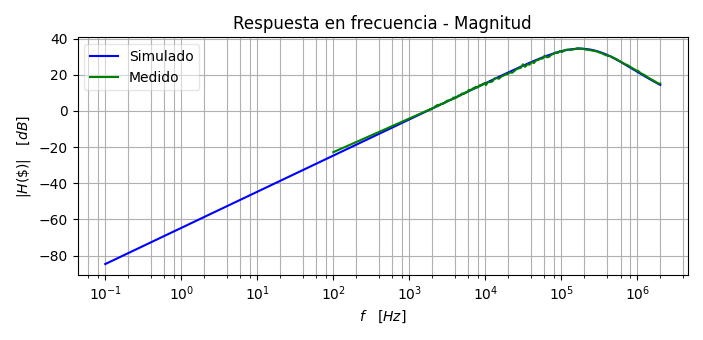
\includegraphics[width=0.6\textwidth]{../Ejercicio3-CircuitoIntegradoresyDerivadores/Imagenes/Derivador/trans_compensa_mag.png}
    \caption{Transferencia compensada - Diagrama de magnitud}

\end{figure}\begin{figure}[H]
    \centering
    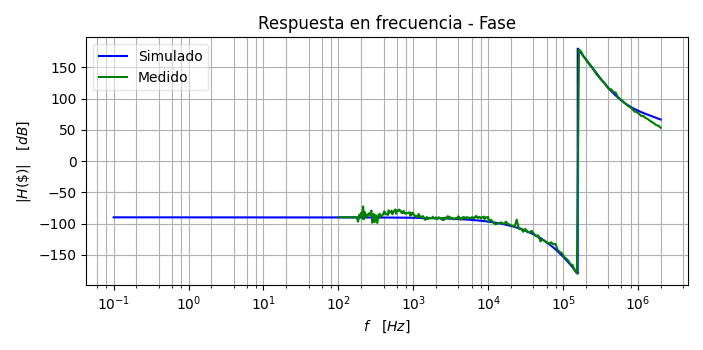
\includegraphics[width=0.6\textwidth]{../Ejercicio3-CircuitoIntegradoresyDerivadores/Imagenes/Derivador/trans_compensa_pha.png}
    \caption{Transferencia compensada - Diagrama de fase}

\end{figure}
Como es de esperar, la transferencia compensada medida coincide con la simulada para nuestro modelo de amplificador 
operacional. Consiguientemente, se procede a comparar los dos sistemas, con y sin compensación.
\begin{figure}[H]
    \centering
    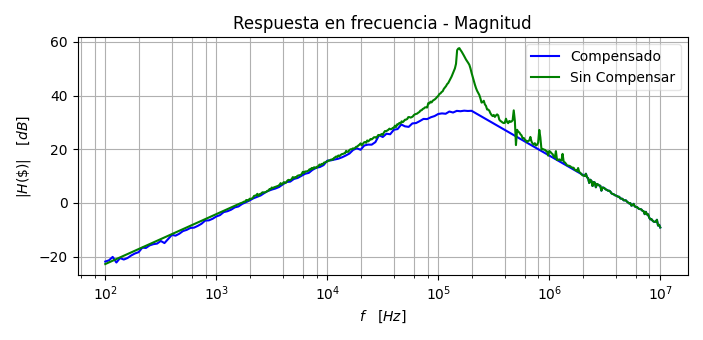
\includegraphics[width=0.6\textwidth]{../Ejercicio3-CircuitoIntegradoresyDerivadores/Imagenes/Derivador/trans_compensa__comp_mag.png}
    \caption{Comparación de las transferencias - Diagrama de magnitud}

\end{figure}\begin{figure}[H]
    \centering
    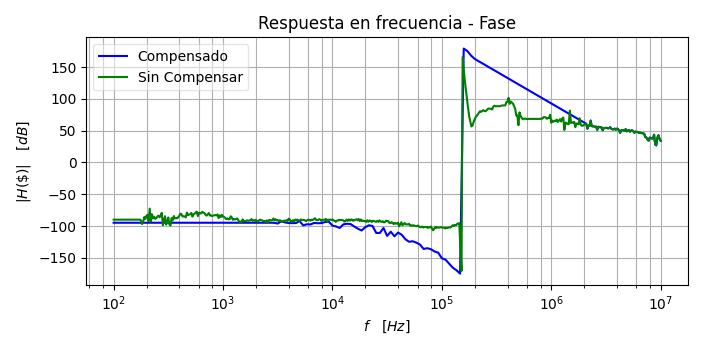
\includegraphics[width=0.6\textwidth]{../Ejercicio3-CircuitoIntegradoresyDerivadores/Imagenes/Derivador/trans_compensa__comp_pha.png}
    \caption{Comparación de las transferencias - Diagrama de fase}

\end{figure}
Como conclusión, se puede afirmar que la compensación se produjo con éxito, teniendo como 
resultado un sistema con menor sobrepico, produciéndose una atenuación de aproximadamente
$30dB$ para dicha frecuencia, otorgandole a la respuesta en frecuencia del circuito mayor 
estabilidad. Por otro lado, el agregado 
de la $R_C$ no modifica la transferencia del circuito original, comportándose de igual manera 
a frecuencias menores a los $150KHz$, zona de interés para el uso de nuestro derivador. \par 
Respecto a la fase, no se observan cambio alguno en la fase de ambos sistemas respecto a la frecuencia para 
la cual el desfasaje es $90^\circ$. Sin embargo, la presencia de $R_C$ suaviza el cambio de fase respecto a los
valores medidos en su ausencia.







\subsection{Circuito Integrador}

\subsubsection{Introducción}

Se realizó el análisis de un circuito integrador con amplificador operacional, utilizando los mismos elementos
que para el caso del circuito derivador pero dispuestos de la siguiente manera:

\begin{figure}[H]
    \centering 
    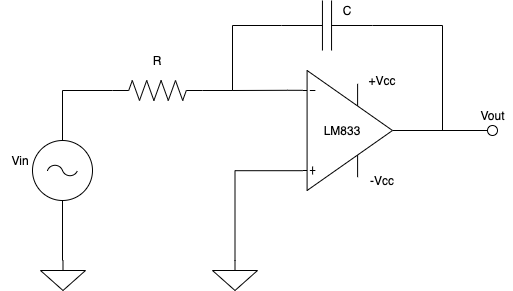
\includegraphics [scale=0.5] {../Ejercicio3-CircuitoIntegradoresyDerivadores/Imagenes/diagrama-integrador.png} 
    \caption{Diagrama del circuito integrador ideal empleado}
    \label{fig:emptyPlotTool}
\end{figure}

A continuación se procederá a calcular teóricamente el valor de las funciones transferencia para los casos en 
donde el amplificador operacional tiene un comportamiento ideal, con $A_{vol}$ finito y $A_{vol}(w)$ con polo dominante.

\subsubsection{Análisis de la Transferencia del Circuito Integrador - OPAMP ideal}

Para obtener la función transferencia en este caso, $H(S) = \frac{V_{out} (S)}{V_{in} (S)}$, partiremos de las siguientes condiciones
iniciales para el amplificador operacional:

\begin{itemize}
	\item $A_{vol}: \infty$
	\item $Z_{in}: \infty$
	\item $Z_{out}: 0$
\end{itemize}

\begin{figure}[H]
    \centering 
    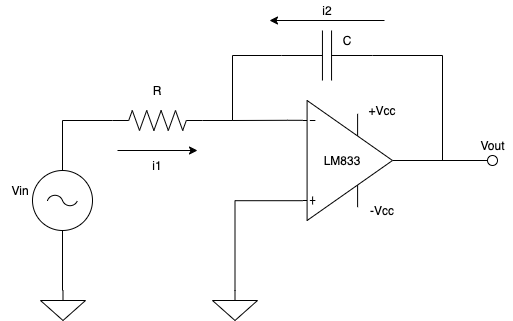
\includegraphics [scale=0.5] {../Ejercicio3-CircuitoIntegradoresyDerivadores/Imagenes/diagrama-integrador-corrientes.png} 
    \caption{Diagrama del circuito integrador ideal empleado}
    \label{fig:emptyPlotTool}
\end{figure}

Podemos observar a simple vista que:

\begin{itemize}
	\item $i1 = -i2$
	\item $i1 = \frac {V_{in}-V^{-}}{R} $
	\item $i2 = \frac {V_{out}-V^{-}}{X_c}$
	\item $V_{out} = A_{vol}(V^{+}-V^{-})$
\end{itemize}

Como ${A_{vol} \to \infty}$ y $V_{out}$ es finito, ${(V^{+}-V^{-}) \to 0}$ y como $V^{+}$ está conectado a tierra,
$V^{-}$ representa tierra virtual, por lo cual su valor es de $0V$.

Entonces, redefiniendo las ecuaciones anteriores:

\begin{itemize}
	\item $i1 = \frac{V_{in}}{R} $
	\item $i2 = \frac {V_{out}}{X_c}$
\end{itemize}

Siendo entonces:

$$ \frac{V_{in}}{R} = - (\frac{V_{out}}{X_c}) \Longrightarrow \frac{V_{out}}{V_{in}} = -\frac{X_c}{R} = - \frac{1}{SRC}$$

$$ H(S) = - \frac{1}{SRC}$$

Queda demostrado teóricamente el comportamiento del sistema como integrador en todo el rango de frecuencias, ya que si antitransformamos la función de transferencia
obtenida implicará que para obtener $v_{out}(t)$ habrá que integrar $v_{in}(t)$ en el dominio del tiempo por tener el factor en el dominio de Laplace de $L(S)=\frac{1}{S}$.
Luego se demostrará que por otras limitaciones, el circuito no funcionará como integrador en todo el rango de frecuencias.

\begin{figure}[H]
    \centering 
    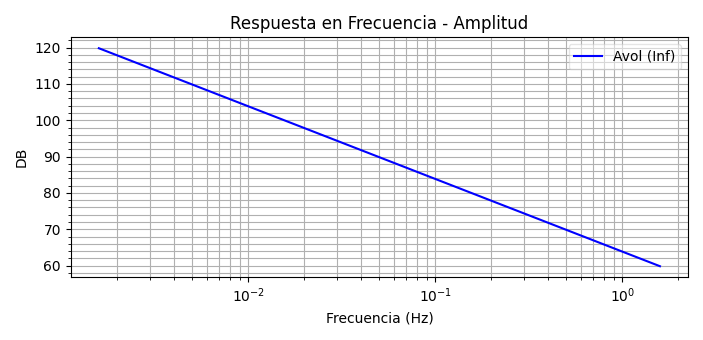
\includegraphics [scale=0.6] {../Ejercicio3-CircuitoIntegradoresyDerivadores/Imagenes/teorico-avol-inf-integrador-amplitud.png} 
    \caption{Respuesta en Frecuencia - Amplitud para OPAMP ideal}
    \label{fig:emptyPlotTool}
\end{figure}

\begin{figure}[H]
    \centering 
    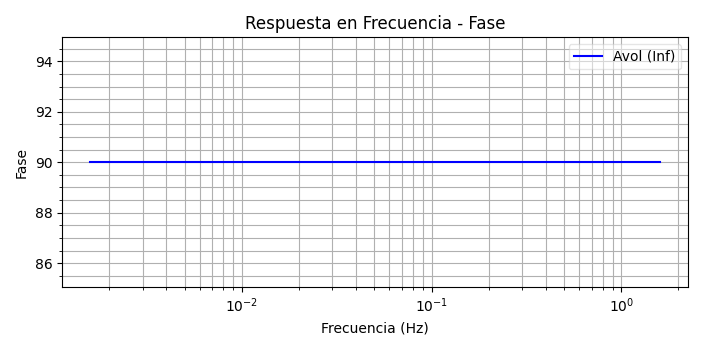
\includegraphics [scale=0.6] {../Ejercicio3-CircuitoIntegradoresyDerivadores/Imagenes/teorico-avol-inf-integrador-fase.png} 
    \caption{Respuesta en Frecuencia - Fase para OPAMP ideal}
    \label{fig:emptyPlotTool}
\end{figure}

\subsubsection{Análisis de la Transferencia del Circuito Integrador - OPAMP con $A_{vol}$ finito}

A diferencia del caso anterior, para el cálculo de la función transferencia, $H(S) = \frac{V_{out} (S)}{V_{in} (S)}$, partiremos de las condiciones planteadas previamente, excepto
:

\begin{itemize}
	\item $A_{vol}: finito$
\end{itemize}

Utilizando entonces las mismas relaciones, se puede observar ahora que:


$$V_{out}=-A_{vol}.V^{-} \Longrightarrow V^{-} = \frac{-V_{out}}{A_{vol}}$$ 


Por lo tanto:

\begin{itemize}
	\item $i1 = \frac {V_{in}-V^{-}}{R} =  \frac {V_{in} + \frac{V_{out}}{A_{vol}}}{R}$
	\item $i2 = \frac {V_{out}-V^{-}}{X_c} = \frac {V_{out} + \frac{V_{out}}{A_{vol}}}{X_c}$
\end{itemize}

Siendo entonces:

$$ \frac {V_{in} + \frac{V_{out}}{A_{vol}}}{R} = -(\frac {V_{out} + \frac{V_{out}}{A_{vol}}}{X_c})
\Longrightarrow \frac{V_{out}}{V_{in}} = \frac{-1}{SCR(1+\frac{1}{A_{vol}}+\frac{1}{A_{vol}SRC})} = \frac{-1}{SCR(1+\frac{1}{A_{vol}})+\frac{1}{A_{vol}}}$$

Finalmente:

$$H(S)= \frac{-A_{vol}}{SCR(A_{vol}+1)+1}$$

Es importante notar que siendo la ganancia para el caso ideal, donde $A_{vol}$ es $\infty$, $ GI = - \frac{1}{SRC}$,  la función
transferencia se puede representar para este caso como $H(S) = GI. \frac{-A_{vol}}{SCR(A_{vol}+1)+1}$. Y
si $A_{vol}$ es lo suficientemente grande, tendremos la función transferencia ideal nuevamente del primer caso analizado para el circuito integrador.

\begin{figure}[H]
    \centering 
    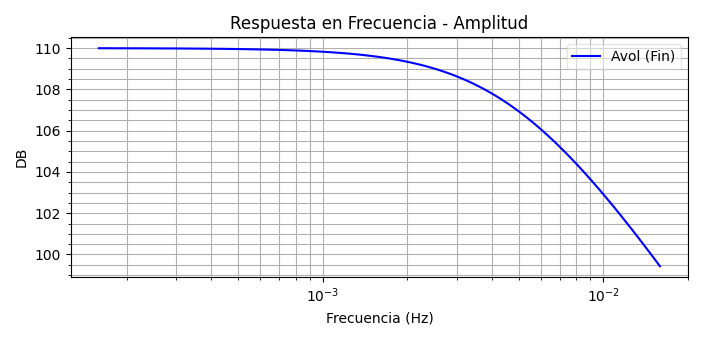
\includegraphics [scale=0.6] {../Ejercicio3-CircuitoIntegradoresyDerivadores/Imagenes/teorico-avol-fin-integrador-amplitud.png} 
    \caption{Respuesta en Frecuencia - Amplitud para OPAMP con $A_{vol}$ finito}
    \label{fig:emptyPlotTool}
\end{figure}

\begin{figure}[H]
    \centering 
    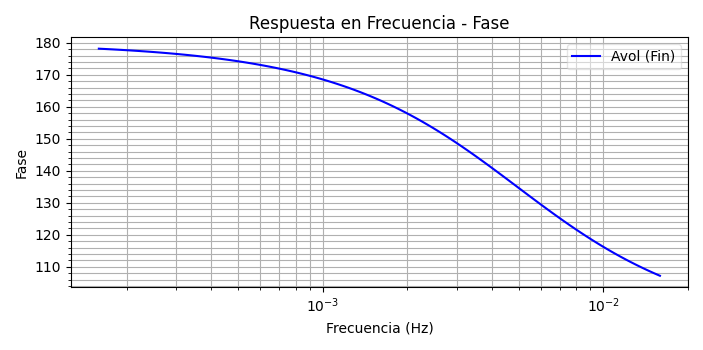
\includegraphics [scale=0.6] {../Ejercicio3-CircuitoIntegradoresyDerivadores/Imagenes/teorico-avol-fin-integrador-fase.png} 
    \caption{Respuesta en Frecuencia - Fase para OPAMP con $A_{vol}$ finito}
    \label{fig:emptyPlotTool}
\end{figure}

\subsubsection{Análisis de la Transferencia del Circuito Integrador - OPAMP con $A_{vol}(w)$}

En este último caso de analisis, $A_{vol}$ no es constante sino que es función de la frecuencia según:

$$A_{vol}(S)=\frac{A_0}{1+\frac{S}{w_b}}$$

Por lo cual utilizando la expresión para la función transferencia calculada en el caso anterior, y evaluando en $A_{vol}(w)$:

$$H(S)= \frac{-1}{SCR(1+\frac{1+\frac{1}{SCR}}{A_{vol}})}\Longrightarrow H(S)= \frac{-1}{SCR(1+\frac{1+\frac{1}{SCR}}{\frac{A_0}{1+\frac{S}{w_b}}})}$$ 

Reacomodando algebraicamente:

$$H(S)=- \frac{1}{S^2\frac{CR}{A_oW_b}+SCR(1 + \frac{1}{A_o}+\frac{1}{W_bA_oCR}) + \frac{1}{A_0}}$$

Finalmente:

$$H(S)=- \frac{{A_0}}{S^2\frac{CR}{W_b}+SCR({A_0} + 1+\frac{1}{W_bCR}) + 1 }$$

Podemos observar que si $A_o$ es muy grande, nuevamente estaremos en el caso donde la ganancia que obtendremos será la ideal para este circuito.

\begin{figure}[H]
    \centering 
    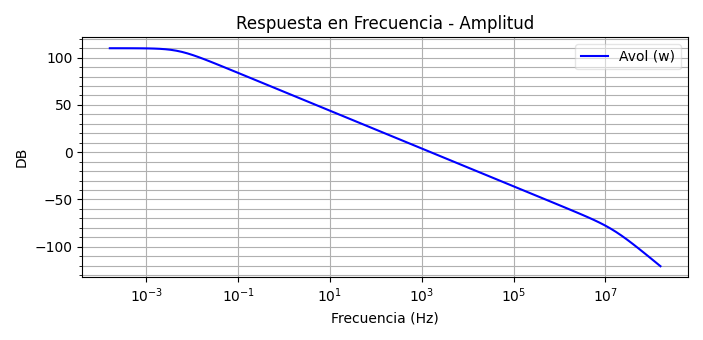
\includegraphics [scale=0.6] {../Ejercicio3-CircuitoIntegradoresyDerivadores/Imagenes/teorico-avol-w-integrador-amplitud.png} 
    \caption{Respuesta en Frecuencia - Amplitud para OPAMP con $A_{vol}(w)$}
    \label{fig:emptyPlotTool}
\end{figure}

\begin{figure}[H]
    \centering 
    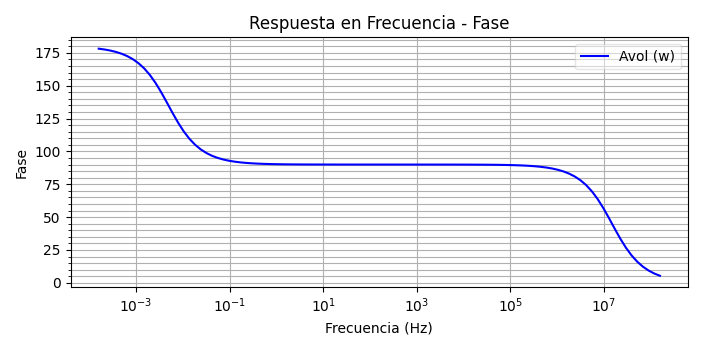
\includegraphics [scale=0.6] {../Ejercicio3-CircuitoIntegradoresyDerivadores/Imagenes/teorico-avol-w-integrador-fase.png} 
    \caption{Respuesta en Frecuencia - Fase para OPAMP con $A_{vol}(w)$ }
    \label{fig:emptyPlotTool}
\end{figure}

Comparando los tres casos, podemos observar que en determinado rango de frecuencias el comportamiento entre los tres casos es muy similar:

%%%%%%
%AGREGAR NUEVOS DIAGRAMAS COMPARATIVOS%

\begin{figure}[H]
    \centering 
    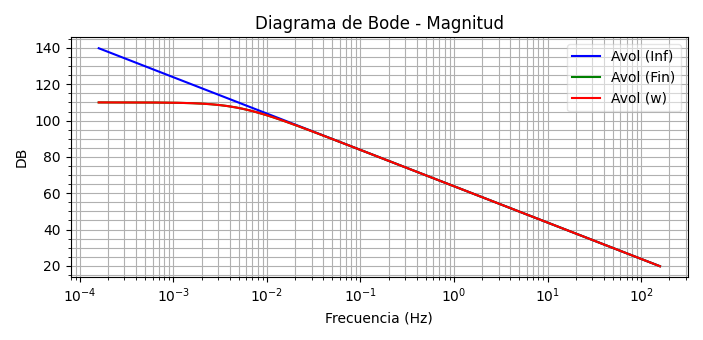
\includegraphics [scale=0.6] {../Ejercicio3-CircuitoIntegradoresyDerivadores/Imagenes/comparativo-magnitud.png} 
    \caption{Respuesta en Frecuencia - Amplitud para los tres modelos de OPAMP }
    \label{fig:emptyPlotTool}
\end{figure}

\begin{figure}[H]
    \centering 
    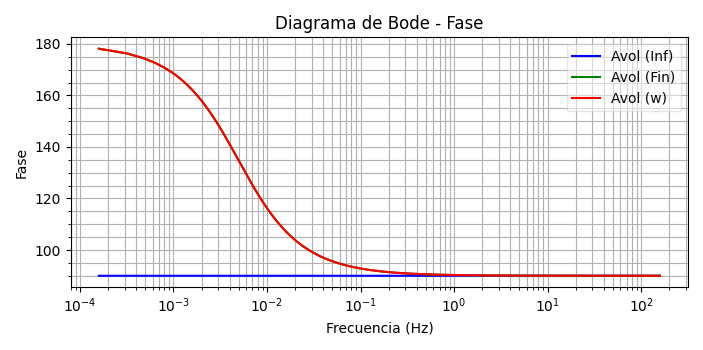
\includegraphics [scale=0.6] {../Ejercicio3-CircuitoIntegradoresyDerivadores/Imagenes/comparativo-fase.png} 
    \caption{Respuesta en Frecuencia - Fase para los tres modelos de OPAMP }
    \label{fig:emptyPlotTool}
\end{figure}

Se puede afirmar que en la intersección de las tres curvas para ambos gráficos, el circuito se comportará como integrador. Para el caso en el que $A_{vol}(w)$, 
observamos el efecto del polo dominante del amplificador operacional en el primer cambio de la fase (aproximadamente en $4.93mHz$). 

Para aportar un valor adicional al análisis y contrastar lo obtenido teóricamente, se realizó la simulación correspondiente en el software $LTSpice$. 
Lo obtenido para la respuesta en frecuencia con los elementos mencionados previamente es:

\begin{figure}[H]
    \centering 
    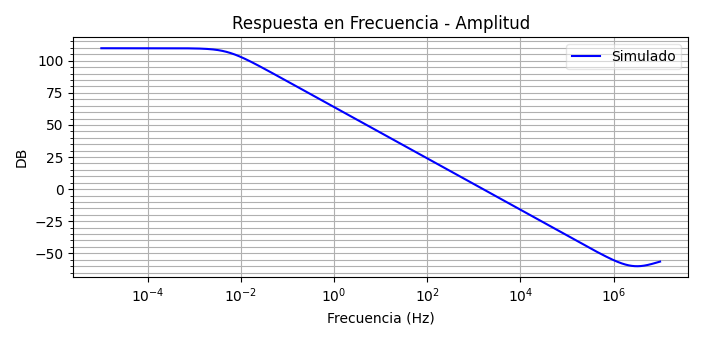
\includegraphics [scale=0.6] {../Ejercicio3-CircuitoIntegradoresyDerivadores/Imagenes/simulado-integrador-amplitud.png} 
    \caption{Respuesta en Frecuencia Simulada - Amplitud para Circuito Integrador }
    \label{fig:emptyPlotTool}
\end{figure}

\begin{figure}[H]
    \centering 
    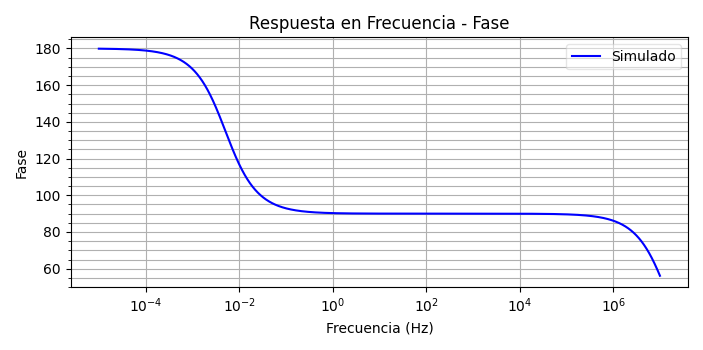
\includegraphics [scale=0.6] {../Ejercicio3-CircuitoIntegradoresyDerivadores/Imagenes/simulado-integrador-fase.png} 
    \caption{Respuesta en Frecuencia Simulada - Fase para Circuito Integrador  }
    \label{fig:emptyPlotTool}
\end{figure}

Se puede observar que los resultados de la simulación muestran total similitud con lo analizado teóricamente para el caso $A_{vol}(w)$.

\subsubsection{Análisis de Entrada Senoidal al circuito integrador}

Se inyectó una señal senoidal variando su amplitud y frecuencia para analizar el comportamiento y la respuesta del circuito.
Se tiene en cuenta que para frecuencias bajas, la ganancia del circuito es alta y podría generar saturación en la salida del circuito $v_{out}(t)$. 
Además de ello, para frecuencias muy altas, la atenuación es tan grande que los valores a analizar se encuentran dentro de los rangos de error de los elementos de medición del
$Electronic$ $Explorer$ $Board$ y a su vez se mezclan con ruido haciendo que las mediciones pierdan precisión.

Como el máximo voltaje posible de alimentación del $Electronic$ $Explorer$ $Board$ es de $\textpm 9V$, no se podrá obtener una amplitud en la señal de salida mayor a dicho voltaje.
En primera instancia, se pudo observar que el circuito cumple su cometido. Integra la señal, es decir, si a la entrada tenemos una señal senoidal, a la salida tendremos una señal cosenoidal de signo opuesto.
En segunda instancia, el circuito amplifica o disminuye la amplitud de la señal de entrada dependiendo esta situación de la frecuencia. 
A frecuencias muy bajas, la señal será amplificada y a frecuencias muy altas, la amplitud se ve reducida, ya que como previamente se mencionó, la ganancia ideal
está determinada por $\frac{-1}{SRC}$.

Partiendo de que para el caso ideal:

$$|H(jw)| = \frac{1}{wRC}$$

Podemos mencionar que teóricamente el circuito atenuará la amplitud de una señal para valores de frecuencia aproximados de:

$$\frac{1}{wRC}\leq 1 \longrightarrow w\geq \frac{1}{RC} \longrightarrow f\geq \frac{1}{2\pi RC}\longrightarrow f \geq 1560 Hz$$

Entonces el circuito aumentará la amplitud de la señal de salida con respecto a la señal de entrada para valores de frecuencia aproximados de:

$$f \leq 1560$$

A medida que la frecuencia disminuye, se puede ver que la ganancia es cada vez mayor pero ésta estará limitada por el valor $A_0$ del amplificador operacional
utilizado que es de $110 DB$ o aproximadamente una ganancia en veces de 316000, valores que nunca serán alcanzados en este caso, ya que no es posible
trabajar con frecuencias tan bajas, tal que se pueda llegar a ese caso y su vez con efectos de saturación aun para amplitudes del orden de los $mV$.

Para ejemplificar lo descripto, se utilizan las siguientes imágenes obtenidas con el Osciloscopio del $Electronic$ $Explorer$ $Board$. En cada caso, se tomó 
la maxima amplitud posible para la frecuencia en la cual se realizaba la medición en la señal inyectada. En el Canal 1, se midió la señal de entrada y en el Canal 2, 
la señal de salida.

En el primer caso se puede observar el desfasaje correspondiente entre las señales y a su vez la gran ganancia en la amplitud de la señal de salida.

\begin{figure}[H]
    \centering 
    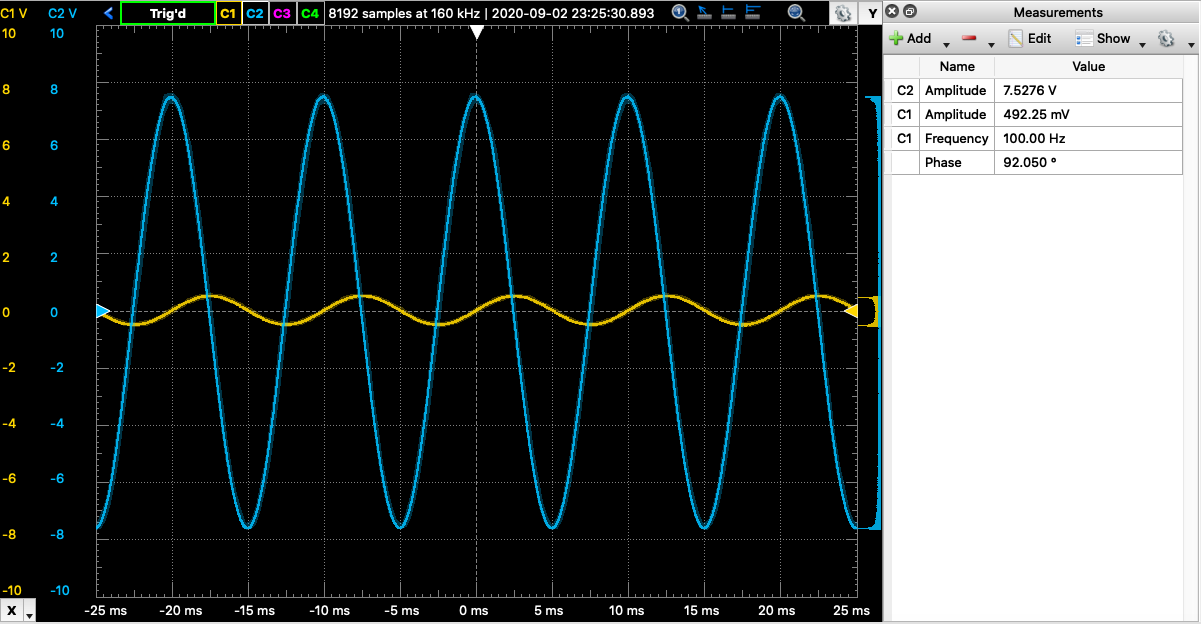
\includegraphics [scale=0.4] {../Ejercicio3-CircuitoIntegradoresyDerivadores/Imagenes/senoidal - 100.png} 
    \caption{Señal de Entrada Senoidal y Señal de Salida - Frecuencia 100 Hz}
    \label{fig:emptyPlotTool}
\end{figure}

En el segundo caso, se pudo observar también el desfasaje pero la ganancia de amplitud ya reducida como era esperado al aumentar la frecuencia.

\begin{figure}[H]
    \centering 
    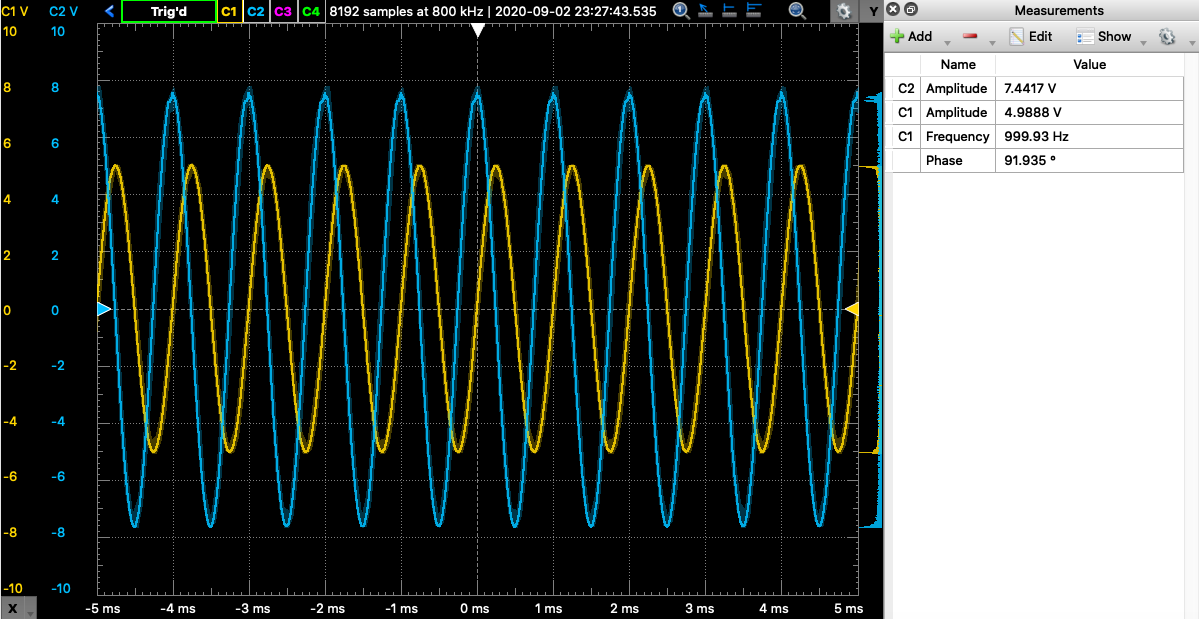
\includegraphics [scale=0.4] {../Ejercicio3-CircuitoIntegradoresyDerivadores/Imagenes/senoidal - 1000.png} 
    \caption{Señal de Entrada Senoidal y Señal de Salida - Frecuencia 1 KHz }
    \label{fig:emptyPlotTool}
\end{figure}

Finalmente, para una frecuencia de $10$ $KHz$, la señal de salida ha reducido notablemente su amplitud en comparación a la señal de entrada.
Además de ello, se observan sobrepicos en la señal de salida.

\begin{figure}[H]
    \centering 
    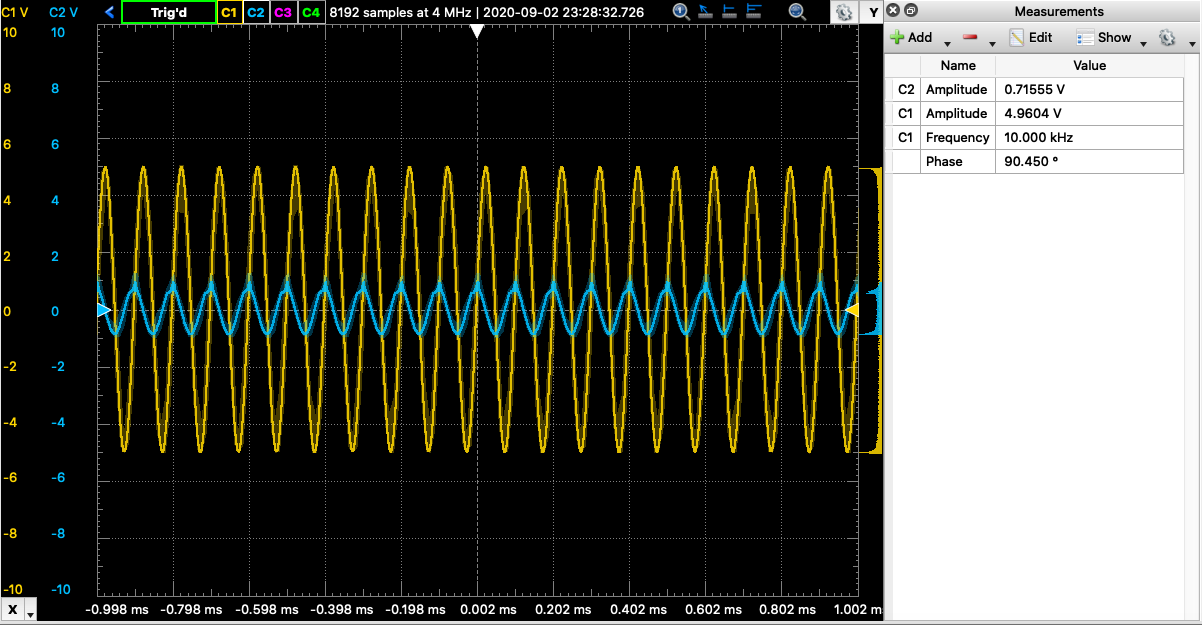
\includegraphics [scale=0.4] {../Ejercicio3-CircuitoIntegradoresyDerivadores/Imagenes/senoidal - 10000.png} 
    \caption{Señal de Entrada Senoidal y Señal de Salida - Frecuencia 10.000 Hz}
    \label{fig:emptyPlotTool}
\end{figure}

Para realizar el diagrama de respuesta en frecuencia no se pudo utilizar la funcionalidad $Network$ del software $WaveForms$ ya que al realizar un barrido en frecuencia
con la misma amplitud para todos los casos, para el rango de frecuencias deseado, en las bajas frecuencias, el sistema saturaría para determinada amplitud y para las frecuencias muy altas, la amplitud de la señal a la salida
está en el orden del error presentado por el osciloscopio del $Electronic$ $Explorer$ $Board$ y se mezcla con ruido.

Se realizaron entonces mediciones manuales, variando la amplitud según la frecuencia, convenientemente, y resultó comparable (en las frecuencias donde se pudo realizar las mediciones)
a los modelos simulado y teórico.

\begin{figure}[H]
    \centering 
    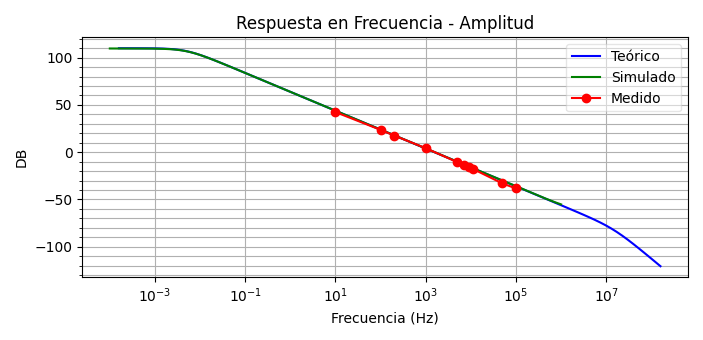
\includegraphics [scale=0.6] {../Ejercicio3-CircuitoIntegradoresyDerivadores/Imagenes/comparativo-integrador-amplitud.png} 
    \caption{Respuesta en Frecuencia Comparativa - Amplitud para Circuito Integrador }
    \label{fig:emptyPlotTool}
\end{figure}

\begin{figure}[H]
    \centering 
    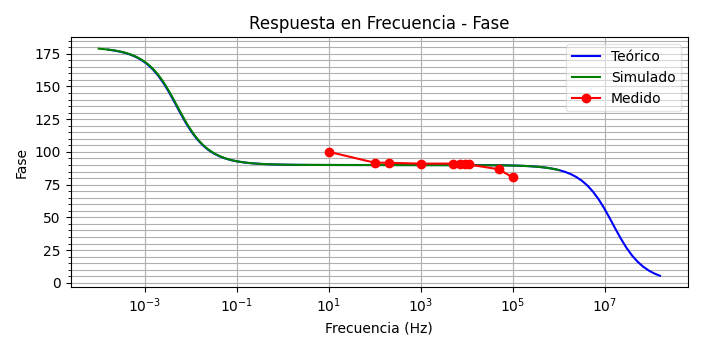
\includegraphics [scale=0.6] {../Ejercicio3-CircuitoIntegradoresyDerivadores/Imagenes/comparativo-integrador-fase.png} 
    \caption{Respuesta en Frecuencia Comparativa - Fase para Circuito Integrador}
    \label{fig:emptyPlotTool}
\end{figure}

Es importante destacar que para frecuencias menores al valor de frecuencia donde se atenua la señal, solo se pudieron realizar mediciones en cierto rango,
ya que la ganancia era tanta que la señal de salida saturaba por superar la maxima tension posible a la salida para este caso que es de aproximidamente $\pm 9V$.
En esos casos, lamentablemente no se pudieron realizar mediciones aun utilizando el rango de los $mV$.

\subsubsection{Análisis de Entrada Cuadrada al Circuito Integrador}

Es importante antes de realizar el análisis para la correspondiente señal de entrada, analizar el comportamiento del capacitor en los distintos rangos de frecuencia.
A medida que la frecuencia se reduce, se puede notar que la magnitud de la señal de salida se ve amplificada pero a su vez, la impedancia representada por el capacitor
también, ya que $X_c= \frac{1}{jwC}$. Al tener una frecuencia lo suficientemente baja, tal que la impedancia $X_c$ es lo suficientemente grande, sucederá que por el cable 
donde está conectado el capacitor no circulará corriente al tener una impedancia extremadamente grande. En otras palabras, allí habrá un circuito abierto.

Al haber un circuito abierto, el proceso de realimentación se verá interrumpido, haciendo que la diferencia mencionada en incisos anteriores que determinaba a 
$v_{out}=A_0(V^+-V^-)$ sea cada ves más grande. Esto guarda correlación con que el hecho de que si baja la frecuencia, la señal de salida se verá más y más amplificada,
y a su vez la diferencia de potencial $(V^+-V^-)$ será cada vez mayor, por estar $V^+$ conectada a tierra y por el hecho de que la retroalimentación del circuito se ve afectada
por la alta impedancia del capacitor e interrumple su ciclo.

Otro factor importante a tener en cuenta es que en el mundo real, los generadores de señales, incluido el generador de señales del $Electronic$ $Explorer$ $Board$ no son ideales,
por lo cual en ellos se presenta una componente de tensión continua que puede ser de mayor o menor valor. La particularidad de este circuito integrador es que amplifica las componentes 
espectrales de frecuencia baja por lo cual, dicha componente de tensión continua se verá amplificada notablemente generando un offset en la señal de salida.

Para poder realizar mediciones con mayor sencillez, se ha utilizado la funcionalidad $Scope$ pero empleando la terminal $AC$ para filtrar dicha componente continua y así evitar
esa tensión de offset. 


A continuación se puede observar el comportamiento integrador del circuito en las frecuencias que así lo permiten.

\begin{figure}[H]
    \centering 
    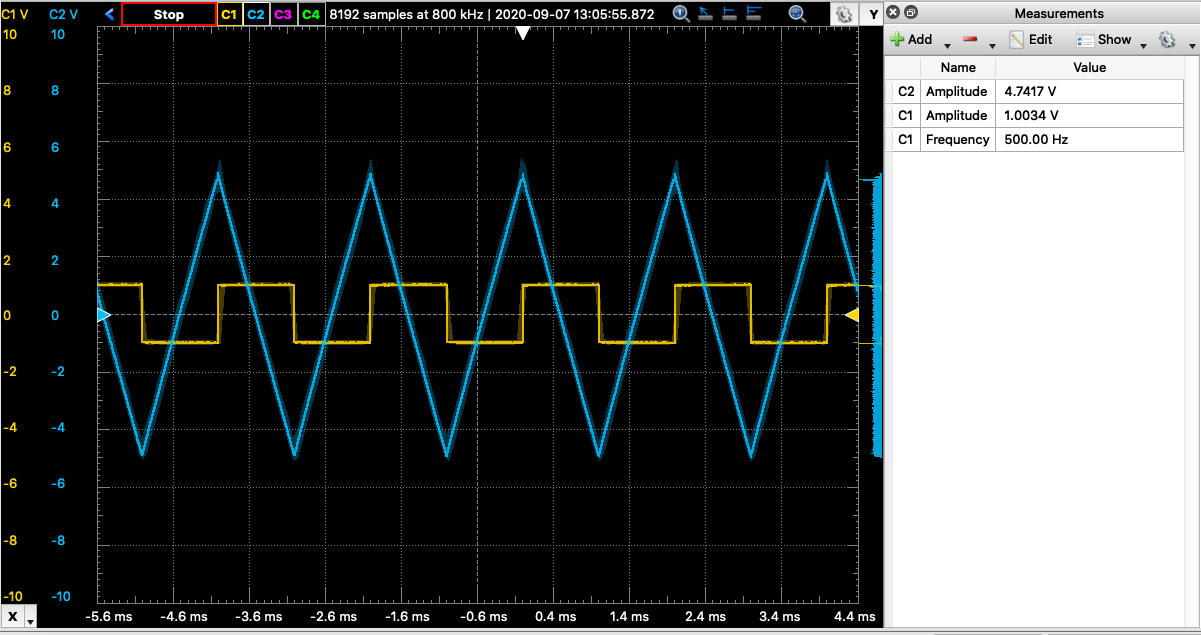
\includegraphics [scale=0.4] {../Ejercicio3-CircuitoIntegradoresyDerivadores/Imagenes/cuadrada-500.png} 
    \caption{Señal de Entrada Cuadrada y Señal Integrada de Salida a 500 Hz }
    \label{fig:emptyPlotTool}
\end{figure}

\begin{figure}[H]
    \centering 
    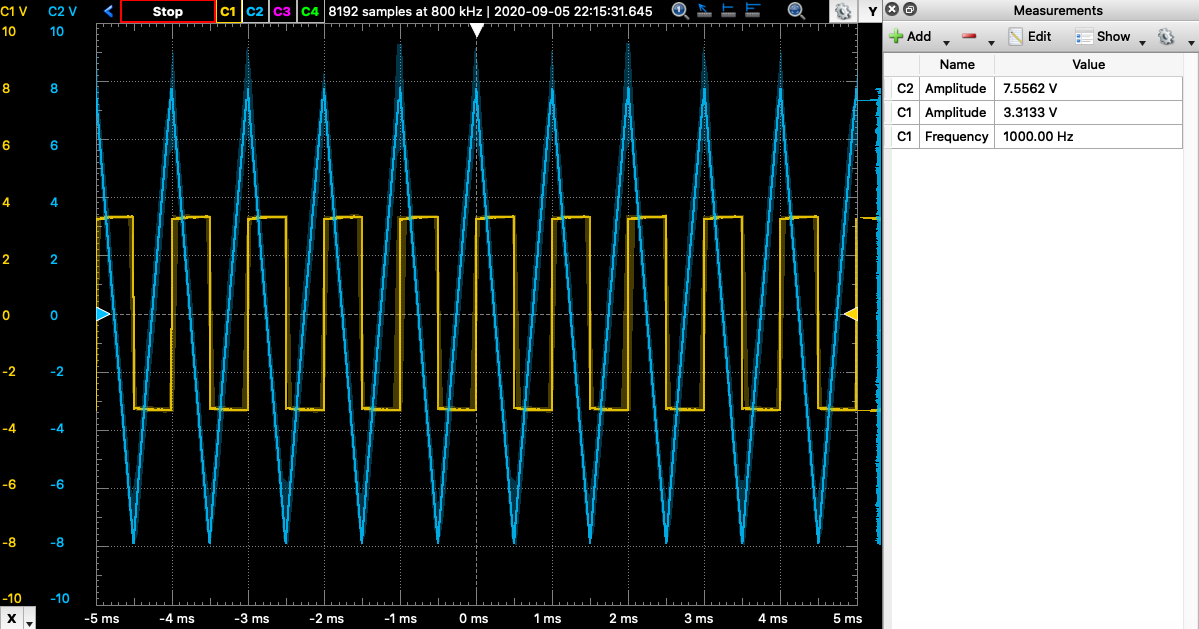
\includegraphics [scale=0.4] {../Ejercicio3-CircuitoIntegradoresyDerivadores/Imagenes/cuadrada-1000.png} 
    \caption{Señal de Entrada Cuadrada y Señal Integrada de Salida a 1 KHz }
    \label{fig:emptyPlotTool}
\end{figure}

\begin{figure}[H]
    \centering 
    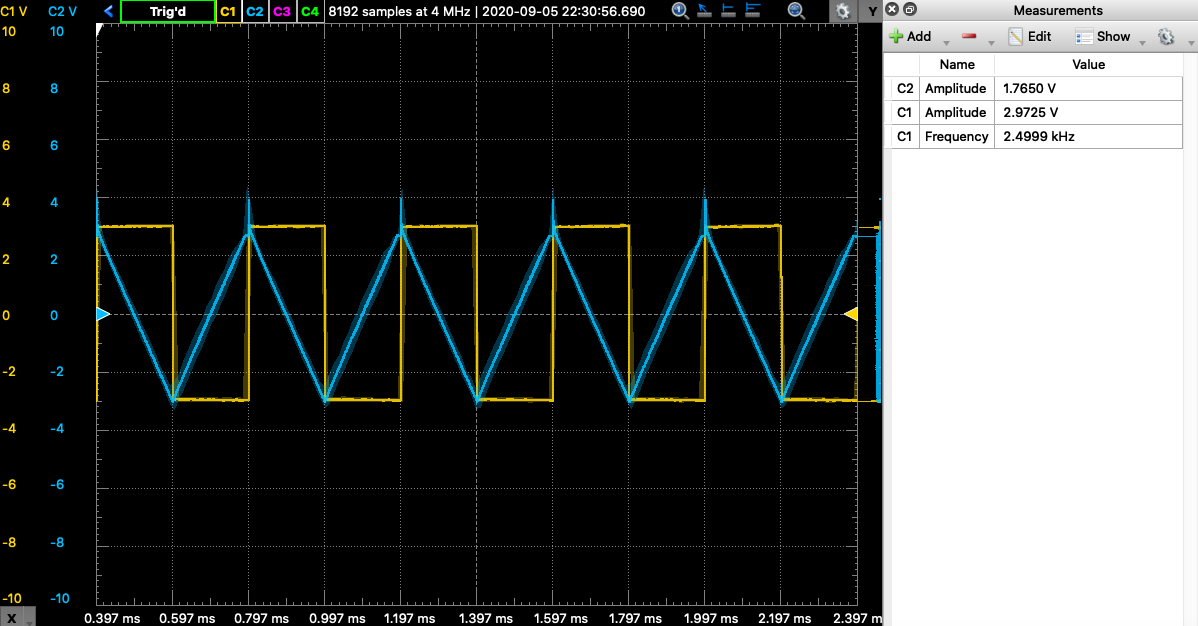
\includegraphics [scale=0.4] {../Ejercicio3-CircuitoIntegradoresyDerivadores/Imagenes/cuadrada-2500.png} 
    \caption{Señal de Entrada Cuadrada y Señal Integrada de Salida a 2.5 KHz}
    \label{fig:emptyPlotTool}
\end{figure}

\begin{figure}[H]
    \centering 
    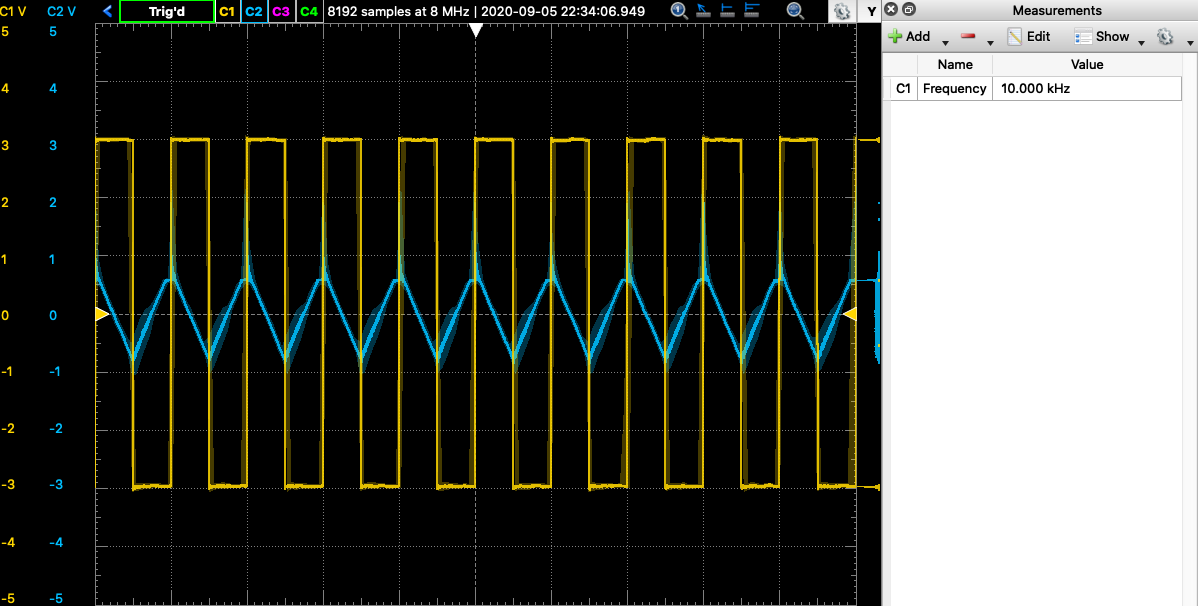
\includegraphics [scale=0.4] {../Ejercicio3-CircuitoIntegradoresyDerivadores/Imagenes/cuadrada-10000.png} 
    \caption{Señal de Entrada Cuadrada y Señal Integrada de Salida a 10 KHz}
    \label{fig:emptyPlotTool}
\end{figure}

En los tres casos, se puede apreciar efectivamente el comportamiento integrador del circuito. Durante los semi-ciclos donde la tensión de la señal 
de la entrada cuadrada es positiva, se puede ver la pendiente negativa en la señal triangular y la situación opuesta se presenta durante el siguiente semi-ciclo.
Ello por el efecto integrador-inversor del circuito.
Además, se observa claramente que a medida que la frecuencia aumenta la amplitud de la señal triangular de salida se atenúa y se pueden también observar
sobrepicos en los gráficos.

\subsubsection{Análisis de Impedancia de Entrada al Circuito Integrador}

Para poder calcular teóricamente la impedancia de entrada, $Z_{in}$, se utilizó el teorema de Miller tal que:

$$ V_{out}=-A_{vol}.V^-$$

Como para este caso, $K=-A_{vol}$, el circuito integrador con el amplificador operacional, queda expresado como:

\begin{figure}[H]
    \centering 
    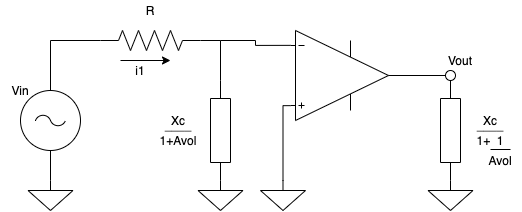
\includegraphics [scale=0.6] {../Ejercicio3-CircuitoIntegradoresyDerivadores/Imagenes/miller-integrador.png} 
    \caption{Diagrama del Circuito Integrador utilizando transformación de Miller }
    \label{fig:emptyPlotTool}
\end{figure}

Como nos interesa $Z_{in}=\frac{V_{in}}{i_1}$, es muy sencillo ver que a la entrada no inversora del amplificador operacional no ingresa corriente,
por lo cual utilizando la ley de tensiones de Kirchoff:

$$ V_{in} = i_1.R + i_1.\frac{X_c}{1+A_{vol}} \longrightarrow \frac{V_{in}}{i_1}= R + \frac{X_c}{1+A_{vol}} \longrightarrow Z_{in}=R+\frac{1}{SC(1+A_{vol})}$$

Dicha impedancia teórica puede verse expresada en las siguientes figuras en conjunto con la expresión simulada mediante $LTSpice$ para ella:

\begin{figure}[H]
    \centering 
    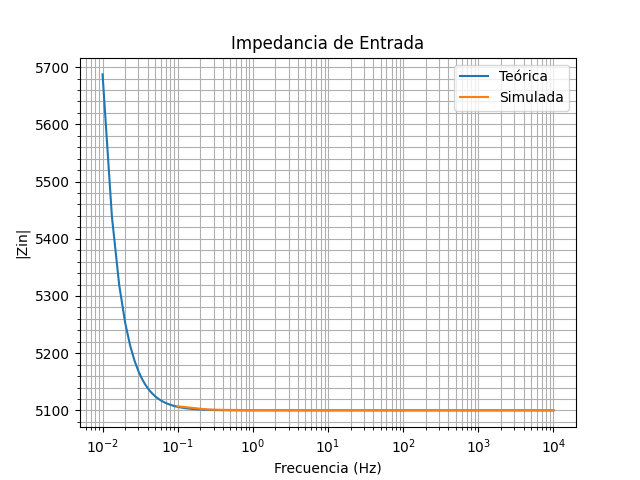
\includegraphics [scale=0.6] {../Ejercicio3-CircuitoIntegradoresyDerivadores/Imagenes/comparativo-integrador-zin-amplitud.png} 
    \caption{Amplitud de $Z_{in}$ en función de $f$}
    \label{fig:emptyPlotTool}
\end{figure}

\begin{figure}[H]
    \centering 
    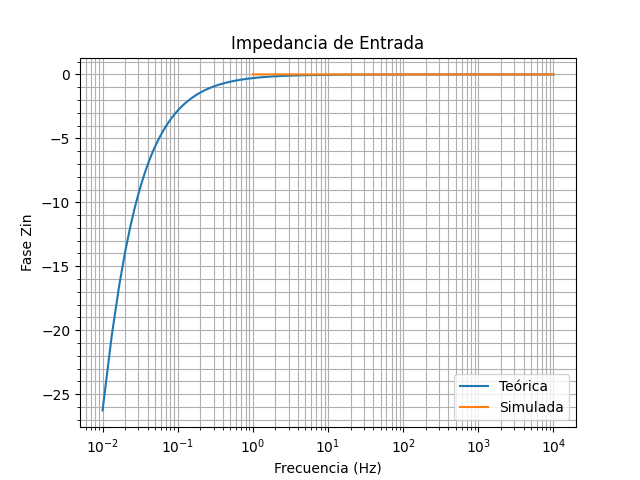
\includegraphics [scale=0.6] {../Ejercicio3-CircuitoIntegradoresyDerivadores/Imagenes/comparativo-integrador-zin-fase.png} 
    \caption{Fase de $Z_{in}$ en función de $f$ }
    \label{fig:emptyPlotTool}
\end{figure}

Se puede observar que a frecuencias bajas, la impedancia tiende a aumentar en magnitud ya que la componente reactiva de 
$Z_{in}$ es inversamente proporcional al valor de la frecuencia como se demostró anteriormente.
A partir de frecuencias del orden de los $Hz$, se puede observar como el efecto de la reactancia capacitiva 
se reduce, dejando unicamente la componente de la $R$. Ello debido a la relación inversa con $A_0$ y con $f$.
Por lo cual podemos afirmar que $Z_{in}$ es aproximadamente $R$ para esos casos.
Lo mismo se puede observar con la fase que tiende a 0, ya que la componente compleja (reactiva) que aporta el capacitor se ve reducida conforme aumenta la frecuencia.
Como conclusión entonces, para aproximadamente $f \geq 1Hz$ :

$$Z_{in} \approx R$$

\subsubsection{Compensación/Limitación del Circuito Integrador con una $R$ adicional}

Como se ha explicado previamente, para el circuito integrador con el amplificador operacional, en frecuencias bajas se interrumpe el ciclo de retroalimentación,
ya que debido a la alta impedancia, en dichas frecuencias, del componente reactivo del circuito, éste se "abre" entre los terminales donde está conectado el capacitor.

Para limitar ese efecto en las bajas frecuencias, es conveniente conectar una resistencia en paralelo al capacitor. El efecto que se logrará es que eligiendo conveniente esa resistencia,
a la que llamaremos $R_c$, se subsanará el efecto de circuito abierto entre las terminales del capacitor a bajas frecuencias. Cuando se "abra" el circuito, la corriente de retroalimentación
aun podrá circular por dicha $R_c$ aunque a su vez, la ganancia del circuito ya no será cada vez mayor a medida que la frecuencia baja, sino que estará limitada por la relación 
$\frac{R_c}{R}$. En ese rango de frecuencias bajas, el circuito integrador actuará como un circuito con amplificador inversor. 

Se pudo observar previamente que la ganancia tendía a $\infty$ conforme la frecuencia disminuía. Ahora en ese rango de frecuencias, la ganancia estará limitada. Por ello, podemos
afirmar que el efecto de agregar la $R_c$ en paralelo al capacitor tendrá un efecto compensatorio para el efecto del capacitor en bajas frecuencias y a su vez limitador en cuanto a la 
ganancia máxima que se podrá obtener, lo cual es un efecto buscado para evitar que la salida $v_{out}$ no sature.

\begin{figure}[H]
    \centering 
    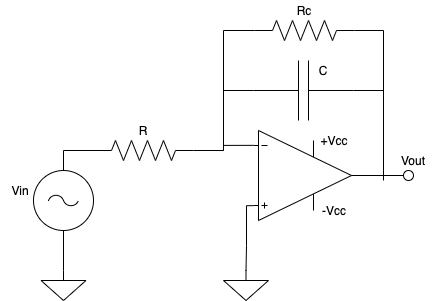
\includegraphics [scale=0.6] {../Ejercicio3-CircuitoIntegradoresyDerivadores/Imagenes/diagrama-integrador-compensado.png} 
    \caption{Diagrama del circuito integrador compensado}
    \label{fig:emptyPlotTool}
\end{figure}

Es conveniente analizar, como será el efecto de esta nueva resistencia introducida en las representaciones de las funciones transferencia para los tres
casos analizados anteriormente. Para ello, simplificaremos el diagrama definiendo a $Z=\frac{X_c.R_c}{X_c+R_c}=\frac{R_c}{SR_cC+1}$

\begin{figure}[H]
    \centering 
    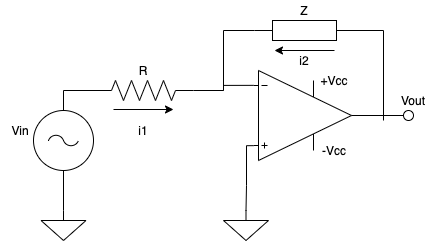
\includegraphics [scale=0.6] {../Ejercicio3-CircuitoIntegradoresyDerivadores/Imagenes/diagrama-integrador-compensado-resumido.png} 
    \caption{Diagrama del circuito integrador compensado con impedancia equivalente para $R_c$ y $C$}
    \label{fig:emptyPlotTool}
\end{figure}

Si $A_{vol} = \infty$:

\begin{itemize}
	\item $i1 = -i2$
	\item $i1 = \frac{V_{in}}{R} $
	\item $i2 = \frac{V_{out}}{Z}$
\end{itemize}

Entonces:

$$ \frac{V_{in}}{R} = - (\frac{V_{out}}{Z}) \Longrightarrow \frac{V_{out}}{V_{in}} = -\frac{Z}{R} = - \frac{R_c}{R}.\frac{1}{SCR_c+1}$$

$$ H(S) = - \frac{R_c}{R}.(\frac{1}{SCR_c+1})$$

Para el caso donde $A_{vol}$ es finito, utilizando las relaciones descriptas en el análisis sin $R_c$:

\begin{itemize}
	\item $i1 = \frac {V_{in}-V^{-}}{R} =  \frac {V_{in} + \frac{V_{out}}{A_{vol}}}{R}$
	\item $i2 = \frac {V_{out}-V^{-}}{Z} = \frac {V_{out} + \frac{V_{out}}{A_{vol}}}{Z}$
\end{itemize}

Siendo entonces:

$$ \frac {V_{in} + \frac{V_{out}}{A_{vol}}}{R} = -(\frac {V_{out} + \frac{V_{out}}{A_{vol}}}{Z})
\Longrightarrow \frac{V_{out}}{V_{in}} = \frac{-1}{(SCR_c+1)\frac{R}{R_c}(1+\frac{1}{A_{vol}})+\frac{1}{A_{vol}}} = 
-\frac{R_c}{R}\frac{1}{(SCR_c+1)(1+\frac{1}{A_{vol}})+\frac{R_c}{RA_{vol}}} $$

Por lo tanto:

$$H(S)= -\frac{R_c}{R}\frac{1}{(SCR_c+1)(1+\frac{1}{A_{vol}})+\frac{R_c}{RA_{vol}}} $$

Para finalizar este análisis, se calculará la función transferencia cuando $A_{vol}(w)$, siendo esta:

$$H(S)=-\frac{R_c}{R}\frac{1}{S^2(\frac{CR_c}{W_bA_0})+SCR_c(1+\frac{1}{A_0}+\frac{1}{W_bA_0CR_c}+\frac{1}{W_bA_0CR})+1+\frac{1}{A_0}+\frac{R_c}{RA_0}}$$

Se puede observar que para los últimos dos casos, nuevamente si $A_{vol}$ es más y más grande, estaremos en el caso de la ganancia ideal para el circuito compensado
por $R_c$.


Para poder determinar cuál es la $R_c$ a emplear, se buscará obtener un desfasaje de $90^o$ entre la señal de entrada y salida en frecuencias lo más baja posible.
A su vez, la ganancia de $-3DB$ por década, será buscada en esa misma frecuencia.
Contar con ambas caracteristicas implica contar con las características propias del integrador ideal. Y a su vez el efecto de compensación/limitación.


Para poder encontrar ese valor, y partiendo del caso ideal con la resistencia
de compensación, donde $ H(S) = - \frac{R_c}{R}.(\frac{1}{SCR_c+1})$, podemos observar que al introducir la resistencia $R_c$
en paralelo contamos con un nuevo polo en donde el desfasaje cambiará a $90^o$ y obtendremos la ganancia de $-3DB$ que dependerá de la frecuencia que nosotros consideremos como baja y el valor de $R_c$ empleado.
Cabe destacar que mientras menor sea la frecuencia elegida, menor será la limitación de la ganancia del circuito.
Para la función de transferencia ideal, contamos con la expresion de un filtro pasa-bajos pasivo como el analizado en la primera experiencia
de laboratorio. Entonces la frecuencia de corte considerada para tal puede ser expresada como:

$$f_0 = \frac{1}{2\pi R_cC}$$

Una década luego de esa frecuencia, obtendremos el comportamiento deseado propio del integrador, y a su vez la limitación en la ganancia del circuito que evitará posibles saturaciones en $V_{out}$.
Tomaremos como frecuencia de integración inicial $f=1KHz$, por lo cual para observar el efecto propio de un integrador a esta frecuencia, elegiremos como frecuencia
$f=100Hz$, ya que una década luego se observarán los efectos deseados. 

Entonces para obtener $R_c$:

$$R_c \geq \frac {1}{2\pi fC} \longrightarrow R_c \geq \frac {1}{2\pi .100.(20n)}\longrightarrow R_c \geq 79577.47 \Omega $$

Se ha utilizado el valor comercial de resistencia de $R_c=82K\Omega$. Con este valor de $R_c$, teóricamente, se puede demostrar que en frecuencias mayores
a $970 Hz$ el sistema deberá integrar sin efectos adversos y a su vez la máxima ganancia del circuito estará denotada por $\frac {R_c}{R}$ que es el equivalente a
$24.12DB$, cuando antes a medida que las frecuencias se acercaban a $0Hz$, tendían a $110DB$. Se puede observar así nuestro efecto limitador en la ganancia.

Es importante mencionar que se podría haber utilizado una $R_c$ de mayor valor, pero en ese caso la ganancia se hubiese limitado menos generando para un mayor rango de frecuencias bajas
un efecto de gran amplificación y consecuente saturación. Por ello, es que se decidió elegir el valor comercial más cercano al valor teórico obtenido.
Como conclusión, establecemos que se decide limitar el rango de frecuencias donde el circuito trabajará como integrador pero la ganancia se ve limitada a un valor
en el cual no se esperarían saturaciones a la salida del circuito.

A continuación se pueden observar las funciones transferencia para los tres casos descriptos:

\begin{figure}[H]
    \centering 
    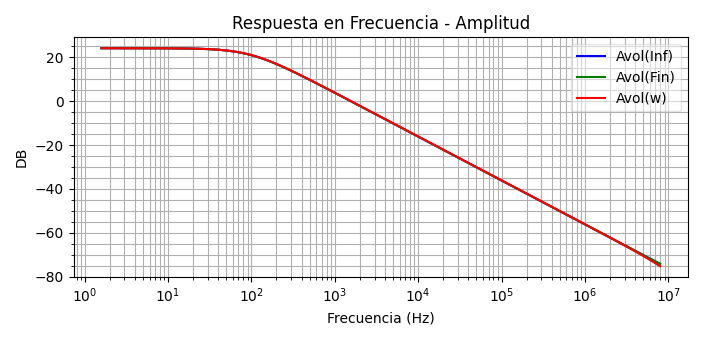
\includegraphics [scale=0.6] {../Ejercicio3-CircuitoIntegradoresyDerivadores/Imagenes/diagrama-bode-integrador-compensado-amplitud.png} 
    \caption{Respuesta en Frecuencia Comparativa - Amplitud para Circuito Integrador Compensado}
    \label{fig:emptyPlotTool}
\end{figure}

\begin{figure}[H]
    \centering 
    \includegraphics [scale=0.6] {../Ejercicio3-CircuitoIntegradoresyDerivadores/Imagenes/diagrama-bode-integrador-compensado-fase.png} 
    \caption{Respuesta en Frecuencia Comparativa - Fase para Circuito Integrador Compensado }
    \label{fig:emptyPlotTool}
\end{figure}

Gráficamente, se puede observar como la ganancia queda limitada ahora al valor de $24.12DB$ para las bajas frecuencias:

\begin{figure}[H]
    \centering 
    \includegraphics [scale=0.6] {../Ejercicio3-CircuitoIntegradoresyDerivadores/Imagenes/diagrama-bode-integrador-compensado-comparativo-amplitud.png} 
    \caption{Respuesta en Frecuencia Comparativa - Amplitud para Circuito Integrador compensado y sin compensar}
    \label{fig:emptyPlotTool}
\end{figure}

\begin{figure}[H]
    \centering 
    \includegraphics [scale=0.6] {../Ejercicio3-CircuitoIntegradoresyDerivadores/Imagenes/diagrama-bode-integrador-compensado-comparativo-fase.png} 
    \caption{Respuesta en Frecuencia Comparativa - Fase para Circuito Integrador compensado y sin compensar }
    \label{fig:emptyPlotTool}
\end{figure}

\subsubsection{Respuesta en Frecuencia del sistema integrador compensado}

Se realizó la simulación del circuito en el software $LTSpice$, obteniendo su respuesta en frecuencia que coincide con lo obtenido teoricamente.

\begin{figure}[H]
    \centering 
    \includegraphics [scale=0.6] {../Ejercicio3-CircuitoIntegradoresyDerivadores/Imagenes/diagrama-bode-integrador-simulado-compensado-amplitud.png} 
    \caption{Respuesta en Frecuencia Simulada - Amplitud para Circuito Integrador compensado}
    \label{fig:emptyPlotTool}
\end{figure}

\begin{figure}[H]
    \centering 
    \includegraphics [scale=0.6] {../Ejercicio3-CircuitoIntegradoresyDerivadores/Imagenes/diagrama-bode-integrador-simulado-compensado-fase.png} 
    \caption{Respuesta en Frecuencia Simulada - Fase para Circuito Integrador compensado }
    \label{fig:emptyPlotTool}
\end{figure}

Además de ello, se realizó la medición de la respuesta en frecuencia utilizando el $Electronic$ $Explorer$ $Board$. Es importante mencionar
que en este caso debido a la limitación en la ganancia, se pudieron realizar mediciones en frecuencias donde antes no era posible por la alta ganancia
en dichas frecuencias que generaban una saturación aún en valores pequeños de amplitud para la señal de entrada.

\begin{figure}[H]
    \centering 
    \includegraphics [scale=0.6] {../Ejercicio3-CircuitoIntegradoresyDerivadores/Imagenes/transferencia-comparativo-todo-amplitud.png} 
    \caption{Respuesta en Frecuencia Comparativa - Amplitud para Circuito Integrador compensado}
    \label{fig:emptyPlotTool}
\end{figure}

\begin{figure}[H]
    \centering 
    \includegraphics [scale=0.6] {../Ejercicio3-CircuitoIntegradoresyDerivadores/Imagenes/transferencia-comparativo-todo-fase.png} 
    \caption{Respuesta en Frecuencia Comparativa - Fase para Circuito Integrador compensado }
    \label{fig:emptyPlotTool}
\end{figure}

Se puede observar que tanto el modelo teórico, simulado y experimental coinciden en su comportamiento. Se puede notar también que
en frecuencias del orden de $1MHz$, al ser tanta la atenuación no es posible medir con precisión la señal de salida y con los elementos con los que 
se cuenta no es posible contrastar empiricamente los tres modelos. Esta misma situación se daba en el circuito sin $R_c$.

En todos los casos medidos, el desfasaje guarda total correlación con los modelos teóricos, sin superar un margen de error de $\textpm$ $3^o$

\subsubsection{Análisis de Entrada Cuadrada al Circuito Integrador Compensado}

Se buscó limitar la ganancia del sistema integrador para evitar efectos de saturación no deseados, pero a su vez, se buscó que el comportamiento integrador
siga siendo el mismo en los rangos donde el circuito sin compensar funcionaba correctamente. Se realizaron las mismas mediciones, y se comprobó que el comportamiento
aun era el esperado.

\begin{figure}[H]
    \centering 
    \includegraphics [scale=0.4] {../Ejercicio3-CircuitoIntegradoresyDerivadores/Imagenes/cuadrada-compensado-1000.png} 
    \caption{Señal de Entrada Cuadrada y Señal Integrada de Salida a 1 KHz para el circuito integrador compensado }
    \label{fig:emptyPlotTool}
\end{figure}

\begin{figure}[H]
    \centering 
    \includegraphics [scale=0.4] {../Ejercicio3-CircuitoIntegradoresyDerivadores/Imagenes/cuadrada-compensado -2500.png} 
    \caption{Señal de Entrada Cuadrada y Señal Integrada de Salida a 2.5 KHz para el circuito integrador compensado }
    \label{fig:emptyPlotTool}
\end{figure}

\begin{figure}[H]
    \centering 
    \includegraphics [scale=0.4] {../Ejercicio3-CircuitoIntegradoresyDerivadores/Imagenes/cuadrada-compensado -10000.png} 
    \caption{Señal de Entrada Cuadrada y Señal Integrada de Salida a 10 KHz para el circuito integrador compensado }
    \label{fig:emptyPlotTool}
\end{figure}

Se puede observar además de que el efecto integrador se mantiene, el efecto integrador se da como se calculó teóricamente,
una década después de la $f_0$ elegida previamente, lo que es equivalente a $1KHz$. 
También donde antes se observaban sobrepicos, ahora ya no están presentes por el efecto compensatorio de $R_c$ .

\subsubsection{Análisis de Impedancia de Entrada al Circuito Integrador compensado}

Para poder calcular teóricamente la impedancia de entrada, $Z_{in}$, para este caso se utilizará también el teorema de Miller tal que:

$$ V_{out}=-A_{vol}.V^-$$

Como para este caso, $K=-A_{vol}$, el circuito integrador con el amplificador operacional, queda expresado como:

\begin{figure}[H]
    \centering 
    \includegraphics [scale=0.6] {../Ejercicio3-CircuitoIntegradoresyDerivadores/Imagenes/miller-integrador-compensado.png} 
    \caption{Diagrama del Circuito Integrador compensado utilizando transformación de Miller }
    \label{fig:emptyPlotTool}
\end{figure}

Como nos interesa $Z_{in}=\frac{V_{in}}{i_1}$, es muy sencillo ver que a la entrada no inversora del amplificador operacional no ingresa corriente,
por lo cual utilizando la ley de tensiones de Kirchoff:

$$ V_{in} = i_1.R + i_1.\frac{Z}{1+A_{vol}} \longrightarrow \frac{V_{in}}{i_1}= R + \frac{Z}{1+A_{vol}} \longrightarrow Z_{in}=R+\frac{R_c}{SCR_c(1+A_{vol})+1+A_{vol}}$$

Dicha impedancia teórica puede verse expresada en las siguientes figuras en conjunto con la expresión simulada mediante $LTSpice$ para ella:

\begin{figure}[H]
    \centering 
    \includegraphics [scale=0.6] {../Ejercicio3-CircuitoIntegradoresyDerivadores/Imagenes/zin-compensado-amplitud.png} 
    \caption{Amplitud de $Z_{in}$ en función de $f$}
    \label{fig:emptyPlotTool}
\end{figure}

\begin{figure}[H]
    \centering 
    \includegraphics [scale=0.6] {../Ejercicio3-CircuitoIntegradoresyDerivadores/Imagenes/zin-compensado-fase.png} 
    \caption{Fase de $Z_{in}$ en función de $f$ }
    \label{fig:emptyPlotTool}
\end{figure}

Se puede observar que en el rango de frecuencias donde se espera el comportamiento integrador del circuito, la impedancia es constante
y equivalente a $R$. Ello se debe al efecto que genera la resistencia de compensacion, en la expresion para $Z_{in}$, en conjunto con 
la relación inversa entre la $f$ y la componente reactiva de $Z_{in}$.

Lo mismo se puede observar con la fase que es 0, ya que la componente reactiva de $Z_{in}$ es mínima aún para frecuencias bajas, debido al efecto
compensatorio de $R_c$

Como conclusión entonces, también para este caso en las frecuencias donde se trabajó:

$$Z_{in} \approx R$$

\subsubsection{Conclusión}

Se pudo observar el comportamiento teórico del circuito integrador con amplificador operacional, a su vez de su comportamiento real.
Es importante destacar de la experiencia, que el comportamiento teórico "menos ideal" coincide con las simulaciones y mediciones realizadas, pero a su vez
el comportamiento integrador ideal no es posible, aunque con la utilización de $R_c$ se implementaron cambios en el circuito para compensar efectos no deseados,
ya sea para controlar la ganancia en la señal de salida, un efecto que dependiendo del uso de este circuito deberá ser menor o peor y también controlar el rango
de comportamiento lineal de este circuito. 

